\part{Programming Techniques}\label{programming-techniques.part}


\chapter{Print Statements and Debugging}

\noindent
Before getting into specific statistical programming techniques
in the following chapters, this chapter is dedicated to comments
and print statements.

\section{Comments}

Stan supports \Cpp-style comments; see \refsection{comments} for full
details.  The recommended style is to use line-based comments for
short comments on the code or to comment out one or more
lines of code.  Bracketed comments are then reserved for long
documentation comments.  The reason for this convention is that
bracketed comments cannot be wrapped inside of bracketed comments.

\subsection{What Not to Comment}

When commenting code, it is usually safe to assume that you are 
writing the comments for other programmers who understand the basics 
of the programming language in use.  In other words, don't comment the
obvious.  For instance, there is no need to have comments
such as the following, which add nothing to the code.
%
\begin{quote}
\begin{Verbatim}
y ~ normal(0,1);  // y has a unit normal distribution
\end{Verbatim}
\end{quote}
%
A Jacobian adjustment for a hand-coded transform might be worth
commenting, as in the following example.
%
\begin{quote}
\begin{Verbatim}
exp(y) ~ normal(0,1);
lp__ <- lp__ + y;  // log Jacobian of exp(y) inverse transform
\end{Verbatim}
\end{quote}
%
It's an art form to empathize with a future code reader and decide
what they will or won't know (or remember) about statistics and Stan.

\subsection{What to Comment}

It can help to document variable declarations if variables are given
generic names like \code{N}, \code{mu}, and \code{sigma}.  For
example, some data variable declarations in an item-response model
might be usefully commented as follows.
%
\begin{quote}
\begin{Verbatim}
int<lower=1> N;   // number of observations
int<lower=1> I;   // number of students
int<lower=1> J;   // number of test questions
\end{Verbatim}
\end{quote}
%
The alternative is to use longer names that do not require comments.
%
\begin{quote}
\begin{Verbatim}
int<lower=1> n_obs;
int<lower=1> n_students;
int<lower=1> n_questions;
\end{Verbatim}
\end{quote}
%
Both styles reasonable and which one to adopt is mostly a matter of
taste (mostly because sometimes models come with their own naming
conventions which should be followed so as not to confuse readers of
the code familiar with the statistical conventions).

Some code authors like big blocks of comments at the top explaining
the purpose of the model, who wrote it, copyright and licensing
information, and so on.  The following bracketed comment is an
example of a conventional style for large comment blocks.
%
\begin{quote}
\begin{Verbatim}
/*
 * Item-Response Theory PL3 Model
 * -----------------------------------------------------
 * Copyright: Joe Schmoe  <joe@schmoe.com>
 * Date:  19 September 2012
 * License: GPLv3
 */

data {
  ...
\end{Verbatim}
\end{quote}
%
The use of leading asterisks helps readers understand the scope of the
comment.  The problem with including dates or other volatile
information in comments is that they can easily get out of synch with
the reality of the code.  A misleading comment or one that is wrong is
worse than no comment at all!

\section{Print Statements}

Stan supports print statements with one or more string or expression
arguments.  Because Stan is an imperative language, variables can have
different values at different points in the execution of a program.
Print statements can be invaluable for debugging, especially for a
language like Stan with no stepwise debugger.

For instance, to print the value of the expression \code{y} along with
the log probability accumulator, use the following statement.
%
\begin{quote}
\begin{Verbatim}
print("y=", y, " log probability=", lp__);
\end{Verbatim}
\end{quote}
%
This print statement prints the string ``y='' followed by the value of
the expression \code{y}, followed by the string `` log probability=''
(with the leading space), followed by the value of the variable
\Verb|lp__|. 

Each print statement is followed by a new line.  The specific ASCII
character(s) generated to create a new line are platform specific.

Arbitrary expressions can be used.  For example, the statement
\begin{quote}
\begin{Verbatim}
print("1+1=", 1+1);
\end{Verbatim}
\end{quote}
%
will print ``1 + 1 = 2'' followed by a new line.

Print statements may be used anywhere other statements may be used,
but their behavior in terms of frequency depends on how often the
block they are in is evaluated.  See \refsection{print-statements} for
more information on the syntax and evaluation of print statements.


\chapter{Missing Data \& Partially Known Parameters}

\noindent
\BUGS and \R support mixed arrays of known and missing data.  In
\BUGS, known and unknown values may be mixed as long as every unknown
variable appears on the left-hand side of either an assignment or
sampling statement.  

\section{Missing Data}


\Stan treats variables declared in the \code{data} and
\code{transformed data} blocks as known and the variables in the
\code{parameters} block as unknown.

The next section shows how to create a mixed array of known and
unknown values as in \BUGS.  The recommended approach to missing data
in \Stan is slightly different than in \BUGS.  An example involving
missing normal observations%
%
\footnote{A more meaningful estimation example would involve a
  regression of the observed and missing observations using predictors
  that were known for each and specified in the \code{data} block.}
%
could be coded as follows.
%
\begin{quote}
\begin{Verbatim}
data {
  int<lower=0> N_obs;
  int<lower=0> N_miss;
  real y_obs[N_obs];
}
parameters {
  real mu;
  real<lower=0> sigma;
  real y_miss[N_miss];
}
model {
  for (n in 1:N_obs)
    y_obs[n] ~ normal(mu,sigma);
  for (n in 1:N_miss)
    y_miss[n] ~ normal(mu,sigma);
}
\end{Verbatim}
\end{quote}
%
The number of observed and missing data points are coded as data with
non-negative integer variables \code{N\_obs} and \code{N\_miss}.  The
observed data is provided as an array data variable \code{y\_obs}.
The missing data is coded as an array parameter, \code{y\_miss}.  The
ordinary parameters being estimated, the location \code{mu} and scale
\code{sigma}, are also coded as parameters.

The model contains one loop over the observed data and one over the
missing data.  This slight redundancy in specification leads to much
more efficient sampling for missing data problems in \Stan than the
more general technique described in the next section.


\section{Partially Known Parameters}\label{partially-known-parameters.section}

In some situations, such as when a multivariate probability function
has partially observed outcomes or parameters, it will be necessary to
create a vector mixing known (data) and unknown (parameter) values.
This can be done in \Stan by creating a vector or array in the
\code{transformed parameters} block and assigning to it.

The following example involves a bivariate covariance matrix in which the
variances are known, but the covariance is not.
%
\begin{quote}
\begin{Verbatim}
data {
  int<lower=0> N;
  vector[2] y[N];
  real<lower=0> var1;     real<lower=0> var2;
}
transformed data {
  real<lower=0> max_cov;  real<lower=0> min_cov;   
  max_cov <- sqrt(var1 * var2);  
  min_cov <- -max_cov;
}
parameters {
  vector[2] mu;
  real<lower=min_cov,upper=max_cov> cov;
}
transformed parameters {
  matrix[2,2] sigma;
  sigma[1,1] <- var1;     sigma[1,2] <- cov;
  sigma[2,1] <- cov;      sigma[2,2] <- var2;
}  
model {
 for (n in 1:N)
   y[n] ~ multi_normal(mu,sigma);
}
\end{Verbatim}
\end{quote}
%
The variances are defined as data in variables \code{var1} and
\code{var2}, whereas the covariance is defined as a parameter in
variable \code{cov}.  The $2 \times 2$ covariance matrix
\code{sigma} is defined as a transformed parameter, with the variances
assigned to the two diagonal elements and the covariance to the two
off-diagonal elements.

The constraint on the covariance declaration ensures that the
resulting covariance matrix \code{sigma} is positive definite.  The
bound, plus or minus the square root of the product of the variances,
is defined as transformed data so that it is only calculated once.

\section{Efficiency Note}

The missing-data example in the first section could be programmed with
a mixed data and parameter array following the approach of the
partially known parameter example in the second section.  The behavior
will be correct, but the computation is wasteful.  Each parameter, be
it declared in the \code{parameters} or \code{transformed parameters}
block, uses an algorithmic differentiation variable which is more
expensive in terms of memory and gradient-calculation time than a
simple data variable.  Furthermore, the copy takes up extra space and
extra time.


\chapter{Truncated or Censored Data}

\noindent
Data in which measurements have been truncated or censored can be
coded in \Stan following their respective probability models.

\section{Truncated Data}

Truncated data is data for which measurements are only reported if
they fall above a lower bound, below an upper bound, or between a
lower and upper bound.  

Truncated data may be modeled in \Stan using truncated distributions.
For example, suppose the truncated data is $y_n$ with an upper
truncation point of $U = 300$ so that $y_n < 300$.  In \Stan, this
data can be modeled as following a truncated normal distribution for
the observations as follows. 
%
\begin{quote}
\begin{Verbatim} 
data {
   int<lower=0> N;
   real U;
   real<upper=U> y[N];
} 
parameters {
   real mu;
   real<lower=0> sigma;
} 
model {
  for (n in 1:N)
       y[n] ~ normal(mu,sigma) T[,U];
}
\end{Verbatim}
\end{quote}
% 
The model declares an upper bound \code{U} as data and constrains
the data for \code{y} to respect the constraint;  this will be checked
when the data is loaded into the model before sampling begins.

This model implicitly uses an improper flat prior on the scale and
location parameters; these could be given priors in the model using
sampling statements.

\subsection{Constraints and Out-of-Bounds Returns}\label{truncation-constraints.section}

If the sampled variate in a truncated distribution lies outside of
the truncation range, the probability is zero, so the log probability
will evaluate to $-\infty$.  For instance, if variate \code{y} is
sampled with the statement.
%
\begin{quote}
\begin{Verbatim}
for (n in 1:N) 
    y[n] ~ normal(mu,sigma) T[L,U];
\end{Verbatim}
\end{quote}
%
then if the value of \code{y[n]} is less than the value of \code{L}
or greater than the value of \code{U}, the sampling statement produces
a zero-probability estimate.

To avoid variables straying outside of truncation bounds, appropriate
constraints are required.  For example, if \code{y} is a parameter in
the above model, the declaration should constrain it to fall between
the values of \code{L} and \code{U}.
%
\begin{quote}
\begin{Verbatim}
parameters {
    real<lower=L,upper=U> y[N];
    ...
\end{Verbatim}
\end{quote}

If in the above model, \code{L} or \code{U} is a parameter and
\code{y} is data, then \code{L} and \code{U} must be appropriately
constrained so that all data is in range and the value of \code{L} is
less than that of \code{U} (if they are equal, the parameter range
collapses to a single point and the Hamiltonian dynamics used by 
the sampler break down).  The following declarations ensure the bounds
are well behaved.
%
\begin{quote}
\begin{Verbatim}
parameters {
    real<upper=min(y)> L; // L < y[n]
    real<lower=fmax(L,max(y))> U; // L < U; y[n] < U
\end{Verbatim}
\end{quote}
%
Note that for pairs of real numbers, the function \code{fmax} is used
rather than \code{max}.







\subsection{Unknown Truncation Points}

If the truncation points are unknown, they may be estimated as
parameters.  This can be done with a slight rearrangement of the
variable declarations from the model in the previous section with
known truncation points.
%
\begin{quote}
\begin{Verbatim}
data {
   int<lower=1> N;
   real y[N];
}
parameters
   real<upper = min(y)> L; 
   real<lower = max(y)> U;
   real mu;
   real<lower=0> sigma;
}
model {
  L ~ ...;  
  U ~ ...;
  for (n in 1:N)
       y[n] ~ normal(mu,sigma) T[L,U];
}
\end{Verbatim}
\end{quote}
%
Here there is a lower truncation point \code{L} which is declared to
be less than or equal to the minimum value of \code{y}.  The upper
truncation point \code{U} is declared to be larger than the maximum
value of \code{y}.  This declaration, although dependent on the data,
only enforces the constraint that the data fall within the truncation
bounds.  With \code{N} declared as type \code{int<lower=1>}, there must be
at least one data point.  The constraint that \code{L} is less than
\code{U} is enforced indirectly, based on the non-empty data.

The ellipses where the priors for the bounds \code{L} and \code{U}
should go should be filled in with a an informative prior in
order for this model to not concentrate \code{L} strongly around 
\code{min(y)} and \code{U} strongly around \code{max(y)}.


\section{Censored Data}

Censoring hides values from points that are too large, too small, or
both.  Unlike with truncated data, the number of data points that were
censored is known.  The textbook example is the household scale which
does not report values above 300 pounds.  

\subsection{Estimating Censored Values}

One way to model censored data is to treat the censored data as
missing data that is constrained to fall in the censored range of
values.  Because \Stan does not allow unknown values in its arrays or
matrices, the censored values must be represented explicitly.
%
\begin{quote}
\begin{Verbatim}
data {
   int<lower=0> N_obs;
   int<lower=0> N_cens;
   real<lower=0> y_obs[N_obs];
   real<lower=max(y_obs)> U;
}
parameters {
  real<lower=U> y_cens[N_cens];
  real mu;
  real<lower=0> sigma;
}
model {
   for (n in 1:N_obs)
       y_obs[n] ~ normal(mu,sigma);
   for (n in 1:N_cens)
       y_cens[n] ~ normal(mu,sigma);
}
\end{Verbatim}
\end{quote}
%
Because the censored data array \code{y\_cens} is declared to be a parameter, it
will be sampled along with the location and scale parameters \code{mu}
and \code{sigma}.  Because the censored data array \code{y\_cens} is
declared to have values of type \code{real<lower=U>}, all imputed values
for censored data will be greater than \code{U}.  The imputed censored
data affects the location and scale parameters through the last
sampling statement in the model.  

\subsection{Integrating out Censored Values}

Although it is wrong to ignore the censored values in estimating
location and scale, it is not necessary to impute values.  Instead,
the values can be integrated out.  Each censored data point has a
probability of
%
\[
\mbox{Pr}[y > U] 
= \int_U^{\infty} \distro{Normal}(y|\mu,\sigma) \, dy
= 1 - \Phi\left(\frac{y - \mu}{\sigma}\right),
\]
%
where $\Phi()$ is the unit normal cumulative distribution function.
With $M$ censored observations, the total probability on the log scale
is
\[
\log \prod_{m=1}^M \mbox{Pr}[y_m > U]
= \log \left( 1 - \Phi\left(\frac{y - \mu}{\sigma}\right)\right)^{M}
= M \, \log \left( 1 - \Phi\left(\frac{y - \mu}{\sigma}\right)\right)
\]
% 
Although \Stan implements $\Phi$ with the function $\code{Phi}$, \Stan
also provides the cumulative distribution function \code{normal\_cdf},
defined by
\[
\code{normal\_cdf}(y,\mu,\sigma) = \Phi \left( \frac{y - \mu}{\sigma} \right).
\]
%
The following model assumes
that the censoring point is known, so it is declared as data.
%
\begin{quote}
\begin{Verbatim}
data {
   int<lower=0> N_obs;
   int<lower=0> N_cens;
   real<lower=0> y_obs[N_obs];
   real<lower=max(y_obs)> U;
}
parameters {
  real mu;
  real<lower=0> sigma;
}
model {
   for (n in 1:N_obs)
       y_obs[n] ~ normal(mu,sigma); 
   lp__ <- lp__ + N_cens * log1m(normal_cdf(U,mu,sigma));
}
\end{Verbatim}
\end{quote}
%
For the observed values in \Verb|y_obs|, the normal sampling model is
used without truncation.  The log probability accumulator
\Verb|lp__| is directly incremented using the calculated log
cumulative normal probability of the censored data items.  The
built-in function \code{log1m} is used, which maps $x$ to $\log (1 -
x)$ in an arithmetically stable way for values of $x$ near zero.

To deal with situations where the censoring point variable \code{U} is
unknown, the declaration of \code{U} should be moved from the data
block to the parameters block.



\chapter{Mixture Modeling}\label{mixture-modeling.chapter}

\noindent
Mixture models of an outcome assume that the outcome is drawn from one
of several distributions, the identity of which is controlled by a
categorical mixing distribution. Mixture models typically have
multimodal densities with modes near the modes of the mixture
components.  Mixture models may be parameterized in several ways,
as described in the following sections.


\section{Latent Discrete Parameterization}

One way to parameterize a mixture model is with a latent categorical
variable indicating which mixture component was responsible for the
outcome. For example, consider $K$ normal distributions with locations
$\mu_k \in \reals$ and scales $\sigma_k \in (0,\infty)$.  Now consider
mixing them in proportion $\theta$, where $\theta_k \geq 0$ and
$\sum_{k=1}^K \theta_k = 1$ (i.e., $\theta$ lies in the unit $K$-simplex).
For each outcome $y_n$ there is a latent variable $z_n$ in
$\setlist{1,\ldots,K}$ with a categorical distribution parameterized
by $\theta$,
%
\[
z_n \sim \distro{Categorical}(\theta).
\]
%
The variable $y_n$ is distributed according to the parameters
of the mixture component $z_n$, 
\[
y_n \sim \distro{Normal}(\mu_{z[n]},\sigma_{z[n]}).
\]
%
This model is not directly supported by \Stan because it involves
discrete parameters $z_n$, but \Stan can sample $\mu$ and $\sigma$ 
by summing out the $z$ parameter as described in the next section.


\section{Summing out the Responsibility Parameter}

To implement the normal mixture model outlined in the previous
section in \Stan, the discrete parameters can be summed out of the
model. If $Y$ is a mixture of $K$ normal distributions with 
locations $\mu_k$ and scales $\sigma_k$ with mixing proportions
$\theta$ in the unit $K$-simplex, then 
\[
p_Y(y) = \sum_{k=1}^K \theta_k \, \distro{Normal}(\mu_k,\sigma_k).
\]

For example, the mixture of $\code{Normal}(-1,2)$ and
$\code{Normal}(3,1)$ with mixing proportion $\theta =
(0.3,0.7)^{\top}$ can be implemented in \Stan as follows.
%
\begin{quote}
\begin{Verbatim}
parameters {
  real y;
}
model {
   lp__ <- log_sum_exp(log(0.3) + normal_log(y,-1,2),
                       log(0.7) + normal_log(y,3,1));
}
\end{Verbatim}
\end{quote}
%
The log probability term is derived by taking
\begin{eqnarray*}
\log p_Y(y) & = & \log \, \left( 0.3 \times \distro{Normal}(y|-1,2) \, + \,
  0.7 \times
  \distro{Normal}(y|3,1) \, \right)
\\[2pt]
& = & \log(\! \begin{array}[t]{l}
                 \exp(\log(0.3 \times \distro{Normal}(y|-1,2))) \\
                 + \exp(\log(0.7 \times \distro{Normal}(y|3,1))) \ )
              \end{array}
% \\[4pt]
% & = & \log( \! \begin{array}[t]{l}\exp(\log(0.3) + \log \distro{Normal}(y|-1,2))
%             \\
%            + \exp(\log(0.7) + \log \distro{Normal}(y|3,1)) \ )
%             \end{array}
\\[2pt]
& = & \mbox{log\_sum\_exp}(\! \begin{array}[t]{l}
                         \log(0.3) + \log \distro{Normal}(y|-1,2),
                         \\                  
                         \log(0.7) + \log \distro{Normal}(y|3,1) \ ).
                       \end{array}
\end{eqnarray*}

Given the scheme for representing mixtures, it may be moved to an
estimation setting, where the locations, scales, and mixture
components are unknown.  Further generalizing to a number of mixture
components specified as data yields the following model.
%
\begin{quote}
\begin{Verbatim}
data {
  int<lower=1> K;          // number of mixture components
  int<lower=1> N;          // number of data points
  real y[N];               // observations
}
parameters {
  simplex[K] theta;        // mixing proportions
  real mu[K];              // locations of mixture components
  real<lower=0,upper=10> sigma[K];  // scales of mixture components
}
model {
  real ps[K];              // temp for log component densities
  for (k in 1:K) {
    mu[k] ~ normal(0,10);
  }
  for (n in 1:N) {
    for (k in 1:K) {
      ps[k] <- log(theta[k]) 
               + normal_log(y[n],mu[k],sigma[k]);
    }
    lp__ <- lp__ + log_sum_exp(ps);    
  }
}
\end{Verbatim}
\end{quote}
%
The model involves \code{K} mixture components and \code{N} data
points. The mixing proportion parameter \code{theta} is declared to be
a unit $K$-simplex, whereas the component location parameter \code{mu}
and scale parameter \code{sigma} are both defined to be arrays of size
\code{K}. The values in the scale array \code{sigma} are constrained
to be non-negative, and have an upper bound of 10. Since no prior is
explicitly defined for the \code{sigma} parameters, their implicit
prior distributions are uniform over their ranges. The model declares
a local array variable \code{ps} to be size \code{K} and uses it to
accumulate the contributions from the mixture components.

The locations and scales are drawn from simple priors for the sake of
this example, but could be anything supported by \Stan.  The mixture
components  could even be modeled hierarchically.

The main action is in the loop over data points \code{n}.  For each
such point, the log of $\theta_k \times
\distro{Normal}(y_n|\mu_k,\sigma_k)$ is calculated and added to the
array \code{ps}.  Then the log probability is incremented with the log
sum of exponentials of those values.





\chapter{Regression Models}

\noindent
\Stan supports regression models from simple linear regressions to
multilevel generalized linear models.  Coding regression models in
\Stan is very much like coding them in \BUGS.

\section{Linear Regression}

The simplest linear regression model is the following, with a single
predictor and a slope and intercept coefficient, and normally
distributed noise.  This model can be written using standard
regression notation as
%
\[
Y_n = \alpha + \beta x_n + \epsilon_n
\ \ \ \mbox{where} \ \ \ 
\epsilon_n \sim \distro{Normal}(0,\sigma).
\]
This is equivalent to the following sampling involving the
residual,
\[
Y_n - (\alpha + \beta X_n) \sim \distro{Normal}(0,\sigma),
\]
and reducing still further, to
\[
Y_n \sim \distro{Normal}(\alpha + \beta X_n, \, \sigma).
\]
%
This latter form of the model is coded in \Stan as follows.
%
\begin{quote}
\begin{Verbatim}
data {
   int<lower=0> N;
   real x[N];
   real y[N];
}
parameters {
    real alpha;
    real beta;
    real<lower=0> sigma;
}
model {
    for (n in 1:N)
        y[n] ~ normal(alpha + beta * x[n], sigma);
}
\end{Verbatim}
\end{quote}
%
There are \code{N} observations, each with predictor \code{x[n]} and
outcome \code{y[n]}.  The intercept and slope parameters are
\code{alpha} and \code{beta}.  The model assumes a normally
distributed noise term with scale \code{sigma}.  This model has
improper priors for the two regression coefficients.

\section{Coefficient and Noise Priors}

There are several ways in which this model can be generalized.  
For example, weak priors can be assigned to the coefficients as follows.
%
\begin{quote}
\begin{Verbatim}
    alpha ~ normal(0,100);
    beta ~ normal(0,100);
\end{Verbatim}
\end{quote}
%
And an upper bound to \code{sigma} can be given in order to implicitly
give it a uniform prior.
\begin{quote}
\begin{verbatim}
    real<lower=0,upper=100> sigma;
\end{verbatim}
\end{quote}

%
More informative priors based the (half) Cauchy distribution are coded
as follows.
%
\begin{quote}
\begin{Verbatim}
    alpha ~ cauchy(0,2.5);
    beta ~ cauchy(0,2.5);
    sigma ~ cauchy(0,2.5);
\end{Verbatim}
\end{quote}
%
The regression coefficients \code{alpha} and \code{beta} are
unconstrained, but \code{sigma} must be positive and properly
requires the half-Cauchy distribution.  Although Stan supports
truncated distributions with half distributions being a special case,
it is not necessary here because the full distribution is proportional
when the parameters are constant.%
%
\footnote{Stan does not (yet) support truncated Cauchy distributions.
  The distributions which may be truncated are listed for discrete
  distributions in \refchapter{discrete-prob-functions} and for
  continuous distributions in \refchapter{continuous-prob-functions}.
  Available truncated distributions may be found in the index by
  looking for suffix \code{\_cdf}.}

\section{Robust Noise Models}

The standard approach to linear regression is to model the noise
term $\epsilon$ as having a normal distribution.  From \Stan's
perspective, there is nothing special about normally distributed
noise.  For instance, robust regression can be accommodated by giving
the noise term a Student-$t$ distribution.  To code this in \Stan, the
sampling distribution is changed to the following.
%
\begin{quote}
\begin{Verbatim}
data {
  ...
  real<lower=0> nu;
}
...
model {
  for (n in 1:N)
    y[n] ~ student_t(nu, alpha + beta * x[n], sigma);
}
\end{Verbatim}
\end{quote}
%
The degrees of freedom constant \code{nu} is specified as data.

\section{Logistic and Probit Regression}\label{logistic-probit-regression.section}

For binary outcomes, either of the closely related logistic or probit
regression models may be used.  These generalized linear models vary
only in the link function they use to map linear predictions in
$(-\infty,\infty)$ to probability values in $(0,1)$.  Their respective
link functions, the logistic function and the unit normal cumulative distribution
function, are both sigmoid functions (i.e., they are both {\it S}-shaped).

A logistic regression model with one predictor and an intercept is coded as
follows.
%
\begin{quote}
\begin{Verbatim}
data {
    int<lower=0> N;
    real x[N];
    int<lower=0,upper=1> y[N];
}
parameters {
    real alpha;
    real beta;
}
model {
    for (n in 1:N)
        y[n] ~ bernoulli(inv_logit(alpha + beta * x[n]));
} 
\end{Verbatim}
\end{quote}
%
The noise parameter is built into the Bernoulli formulation here
rather than specified directly.

Logistic regression is a kind of generalized linear model with binary
outcomes and the log odds (logit) link function.  The inverse of the
link function appears in the model.  

Other link functions may be used in the same way.  For example, probit
regression uses the cumulative normal distribution function, which is
typically written as 
\[
\Phi(x) = \int_{-\infty}^x \distro{Normal}(y|0,1) \, dy.
\]
%
The cumulative unit normal distribution function $\Phi$ is implemented
in \Stan as the function \code{Phi}.  The probit regression model
may be coded in \Stan by replacing the logistic model's sampling
statement with the following.
%
\begin{quote}
\begin{Verbatim}
        y[n] ~ bernoulli(Phi(alpha + beta * x[n]));
\end{Verbatim}
\end{quote}
%
A fast approximation to the cumulative unit normal distribution function 
$\Phi$ is implemented in \Stan as the function \code{Phi\_approx}.  The 
approximate probit regression model may be coded with the following.
%
\begin{quote}
\begin{Verbatim}
        y[n] ~ bernoulli(Phi_approx(alpha + beta * x[n]));
\end{Verbatim}
\end{quote}

\section{Multi-Logit Regression}

Multiple outcome forms of logistic regression can be coded directly in
\Stan.  For instance, suppose there are $K$ possible outcomes for each
output variable $y_n$.  Also suppose that there is a $D$-dimensional
vector $x_n$ of predictors for $y_n$.  The multi-logit model with
$\distro{Normal}(0,5)$ priors on the coefficients is coded as follows.
%
\begin{quote}
\begin{Verbatim}
data {
   int<lower=2> K;
   int<lower=0> N;
   int<lower=1> D;
   int<lower=1,upper=K> y[N];
   vector[D] x[N];
}
parameters {
   matrix[K,D] beta;
}
model {
  for (k in 1:K)
    for (d in 1:D)
      beta[k,d] ~ normal(0,5);
  for (n in 1:N)
     y[n] ~ categorical(softmax(beta * x[n]));
}
\end{Verbatim}
\end{quote}
%
The softmax function is defined for a $K$-vector $\gamma \in \reals^K$ by
\[
\mbox{softmax}(\gamma) = 
\left(
 \frac{\exp(\gamma_1)}
      {\sum_{k=1}^K \exp(\gamma_k)},
  \ldots,
  \frac{\exp(\gamma_K)}
       {\sum_{k=1}^K \exp(\gamma_k)}
\right).
\]
%
The result is in the unit $K$-simplex and thus appropriate to use as
the parameter for a categorical distribution.

\subsection{Identifiability}

Because softmax is invariant under adding a constant to each component
of its input, the model is typically only identified if there is a
suitable prior on the coefficients.

An alternative is to use $K-1$ vectors by fixing one of them to be
zero.  See \refsection{partially-known-parameters} for an example of
how to mix known quantities and unknown quantities in a vector.


\section{Ordered Logistic and Probit Regression}\label{ordered-logistic.section}

Ordered regression for an outcome $y_n \in \setlist{1,\ldots,K}$ with
predictors $x_n \in \reals^D$ is determined by a single coefficient
vector $\beta \in \reals^D$ along with a sequence of cutpoints $c \in
\reals^{D-1}$ sorted so that $c_d < c_{d+1}$.  The discrete output is
$k$ if the linear predictor $x_n \beta$ falls between $c_{k-1}$ and
$c_k$, assuming $c_0 = -\infty$ and $c_K = \infty$.  The noise term is
fixed by the form of regression, with examples for ordered logistic
and ordered probit models.  

\subsection{Ordered Logistic Regression}

The ordered logistic model can be coded in \Stan using the
\code{ordered} data type for the cutpoints and the built-in
\code{ordered\_logistic} distribution.
%
\begin{quote}
\begin{Verbatim} 
data {
  int<lower=2> K;
  int<lower=0> N;
  int<lower=1> D;
  int<lower=1,upper=K> y[N];
  row_vector[D] x[N];
} 
parameters {
  vector[D] beta;
  ordered[K-1] c;
} 
model {
  for (n in 1:N)
      y[n] ~ ordered_logistic(x[n] * beta, c);
}
\end{Verbatim}
\end{quote}
% 
The vector of cutpoints \code{c} is declared as \code{ordered[K-1]},
which guarantees that \code{c[k]} is less than \code{c[k+1]}. 

If the cutpoints were assigned independent priors, the constraint
effectively truncates the joint prior to support over points that
satisfy the ordering constraint.  Luckily, \Stan does not need to
compute the effect of the constraint on the normalizing term because
the probability is only needed up to a proportion.


\subsubsection{Ordered Probit}

An ordered probit model could be coded in a manner similar to the
\BUGS encoding of an ordered logistic model.
%
\begin{quote}
\begin{Verbatim}
data {
  int<lower=2> K;
  int<lower=0> N;
  int<lower=1> D;
  int<lower=1,upper=K> y[N];
  row_vector[D] x[N];
}
parameters {
  vector[D] beta;
  ordered[K-1] c;
}
model {
  vector[K] theta;
  for (n in 1:N) {
      real eta;
      eta <- x[n] * beta;
      theta[1] <- 1 - Phi(eta - c[1]);
      for (k in 2:(K-1))
          theta[k] <- Phi(eta - c[k-1]) - Phi(eta - c[k]);
      theta[K] <- Phi(eta - c[K-1]);
      y[n] ~ categorical(theta);
  }
}
\end{Verbatim}
\end{quote}
%
The logistic model could also be coded this way by replacing
\code{Phi} with \code{inv\_logit}, though the built-in encoding based
on the softmax transform is more efficient and more numerically
stable.  A small efficiency gain could be achieved by computing the
values \code{Phi(eta - c[k])} once and storing them for re-use.

\section{Hierarchical Logistic Regression}

The simplest multilevel model is a hierarchical model in which the
data is grouped into $L$ distinct categories (or levels).  An extreme approach would be to
completely pool all the data and estimate a common vector of
regression coefficients $\beta$.  At the other extreme, an approach
would no pooling assigns each level $l$ its own coefficient vector
$\beta_l$ that is estimated separately from the other levels.  A
hierarchical model is an intermediate solution where the degree of
pooling is determined by the data and a prior on the amount of
pooling.

Suppose each binary outcome $y_n \in \setlist{0,1}$ has an associated
level, $ll_n \in \setlist{1,\ldots,L}$.  Each outcome will also have
an associated predictor vector $x_n \in \reals^D$.  Each level $l$
gets its own coefficient vector $\beta_l \in \reals^D$.  The
hierarchical structure involves drawing the coefficients $\beta_{l,d}
\in \reals$ from a prior that is also estimated with the data.  This
hierarchically estimated prior determines the amount of pooling.  If
the data in each level are very similar, strong pooling will be
reflected in low hierarchical variance.  If the data in the levels are
dissimilar, weaker pooling will be reflected in higher hierarchical variance.

The following model encodes a hierarchical logistic regression model
with a hierarchical prior on the regression coefficients.
%
\begin{quote}
\begin{Verbatim}
data {
    int<lower=1> D;
    int<lower=0> N;
    int<lower=1> L;
    int<lower=0,upper=1> y[N];
    int<lower=1,upper=L> ll[N];
    row_vector[D] x[N];
}
parameters {
    real mu[D];
    real<lower=0,upper=1000> sigma[D];
    vector[D] beta[L];
}
model {
    for (d in 1:D) {
        mu[d] ~ normal(0,100);
        for (l in 1:L)
            beta[l,d] ~ normal(mu[d],sigma[d]);
    }
    for (n in 1:N)
        y[n] ~ bernoulli(inv_logit(x[n] * beta[ll[n]]));
}
\end{Verbatim}
\end{quote}   


\section{Item-Response Theory Models}

Item-response theory (IRT) models the situation in which a number of
students each answer one or more of a group of test questions.  The
model is based on parameters for the ability of the students, the
difficulty of the questions, and in more articulated models, the
discimrinativess of the questions and the probability of guessing
correctly; see \citep[pps.~314--320]{GelmanHill:2007} for a textbook
introduction to hierarchical IRT models and \citep{Curtis:2010} for
encodings of a range of IRT models in BUGS.


\subsection{Data Declaration with Missingness}

The data provided for an IRT model may be declared as follows
to account for the fact that not every student is required to answer
every question.
%
\begin{quote}
\begin{Verbatim}
data {
  int<lower=1> J;              // number of students
  int<lower=1> K;              // number of questions
  int<lower=1> N;              // number of observations
  int<lower=1,upper=J> jj[N];  // student for observation n
  int<lower=1,upper=K> kk[N];  // question for observation n
  int<lower=0,upper=1> y[N];   // correctness for observation n
}
\end{Verbatim}
\end{quote}
%
This declares a total of \code{N} student-question pairs in the data
set, where each \code{n} in \code{1:N} indexes a binary observation
\code{y[n]} of the correctness of the answer of student \code{jj[n]}
on question \code{kk[n]}.

The prior hyperparameters will be hard coded in the rest of this
section for simplicity, though they could be coded as data in
Stan for more flexibility.

\subsection{1PL (Rasch) Model}

The 1PL item-response model, also known as the Rasch model, has one
parameter (1P) for questions and uses the logistic link function (L).
This model is distributed with Stan in the file
\url{src/models/misc/irt/irt.stan}.

The model parameters are declared as follows.
%
\begin{quote}
\begin{Verbatim} 
parameters {    
  real delta;         // mean student ability
  real alpha[J];      // ability of student j - mean ability
  real beta[K];       // difficulty of question k
}
\end{Verbatim}
\end{quote}
%
The parameter \code{alpha[j]} is the ability coefficient for student
\code{j} and \code{beta[k]} is the difficulty coefficient for question
\code{k}.  The non-standard parameterization used here also includes
an intercept term \code{delta}, which represents the average student's
response to the average question.%
%
\footnote{\citep{GelmanHill:2007} treat the $\delta$ term equivalently
  as the location parameter in the distribution of student abilities.}
%
The model itself is as follows.
%
\begin{quote}
\begin{Verbatim} 
model {
  alpha ~ normal(0,1);         // informative true prior
  beta ~ normal(0,1);          // informative true prior
  delta ~ normal(.75,1);       // informative true prior
  for (n in 1:N)
    y[n] ~ bernoulli_logit(alpha[jj[n]] - beta[kk[n]] + delta);
}
\end{Verbatim}
\end{quote}
%
This model uses the logit-parameterized Bernoulli distribution, where
\[
\code{bernoulli\_logit}(y|\alpha) =
\code{bernoulli}(y|\mbox{logit}^{-1}(\alpha)).
\]
%
The key to understanding it is the term inside the
\code{bernoulli\_logit} distribution, from which it follows that
\[
\mbox{Pr}[Y_n = 1] = \mbox{logit}^{-1}(\alpha_{jj[n]} - \beta_{kk[n]}
+ \delta).
\]
%
The model suffers from additive identifiability issues without the
priors.  For example, adding a term $\xi$ to each $\alpha_j$ and
$\beta_k$ results in the same predictions.  The use of priors for
$\alpha$ and $\beta$ located at 0 identifies the parameters; see
\citep{GelmanHill:2007} for a discussion of identifiability issues and
alternative approaches to identification.  

For testing purposes, the IRT 1PL model distributed with Stan uses
informative priors that match the actual data generation process used
to simulate the data in R (the simulation code is supplied in the same
directory as the models).  This is unrealistic for most practical
applications, but allows Stan's inferences to be validated.  A simple
sensitivity analysis with fatter priors shows that the posterior is
fairly sensitive to the prior even with 400 students and 100 questions
and only 25\% missingness at random.  For real applications, the
priors should be fit hierarchically along with the other parameters,
as described in the next section.


\subsection{Multilevel 2PL Model}

The simple 1PL model described in the previous section is generalized
in this section with the addition of a discrimination parameter to
model how noisy a question is and by adding multilevel priors for the
student and question parameters.

The model parameters are declared as follows.
%
\begin{quote}
\begin{Verbatim}
parameters {    
  real delta;                  // mean student ability
  real alpha[J];               // ability for j - mean
  real beta[K];                // difficulty for k
  real log_gamma[K];           // discrim for k
  real<lower=0> sigma_alpha;   // sd of abilities
  real<lower=0> sigma_beta;    // sd of difficulties 
  real<lower=0> sigma_gamma;   // sd of log discrim
}
\end{Verbatim}
\end{quote}
%
The parameters should be clearer after the model definition.
%
\begin{quote}
\begin{Verbatim}
model {
  alpha ~ normal(0,sigma_alpha); 
  beta ~ normal(0,sigma_beta);   
  log_gamma ~ normal(0,sigma_gamma);
  delta ~ cauchy(0,5);
  sigma_alpha ~ cauchy(0,5);
  sigma_beta ~ cauchy(0,5);
  sigma_gamma ~ cauchy(0,5);
  for (n in 1:N)
    y[n] ~ bernoulli_logit( 
               exp(log_gamma[kk[n]])
               * (alpha[jj[n]] - beta[kk[n]] + delta) );
}
\end{Verbatim}
\end{quote}
%
First, the predictor inside the \code{bernoulli\_logit} term is
equivalent to the predictor of the 1PL model multipled by the
discriminativeness for the question, \code{exp(log\_gamma[kk[n]])}.
The parameter \code{log\_gamma[k]} represents how discriminative a
question is, with log discriminations above 0 being less (because
their exponentiation drives the predictor away from zero, which drives
the prediction away from 0.5) and discriminations below 0 being more
noisy (driving the predictor toward zero and hence the prediction
toward 0.5).

The intercept term \code{delta} can't be modeled hierarchically, so it
is given a weakly informative $\distro{Cauchy}(0,5)$ prior.
Similarly, the scale terms, \code{sigma\_alpha}, \code{sigma\_beta},
and \code{sigma\_gamma}, are given half-Cauchy priors.  The truncation
in the half-Cauchy prior is implicit; explicit truncation is not
necessary because the log probabilty need only be calculated up to a
proportion and the scale variables are constrained to $(0,\infty)$ by 
their declarations.



\section{Autoregressive Models}

A first-order autoregressive model (AR(1)) with normal noise takes
each point $y_n$ in a sequence $y$ to be generated according to
%
\[
y_n \sim \distro{Normal}(\alpha + \beta y_{n-1}, \sigma).
\]
%
That is, the expected value of $y_n$ is $\alpha + \beta y_{n-1}$, with
noise scaled as $\sigma$.

\subsection{AR(1) Models}

With improper flat priors on the regression coefficients for slope
($\beta$), intercept ($\alpha$), and noise scale ($\sigma$),
the \Stan program for the AR(1) model is as follows.
%
\begin{quote}
\begin{Verbatim}
data {
    int<lower=0> N;
    real y[N];
}
parameters {
    real alpha;
    real beta;
    real sigma;
}
model {
    for (n in 2:N)
       y[n] ~ normal(alpha + beta*y[n-1], sigma);
}
\end{Verbatim}
\end{quote}
%
The first observed data point, \code{y[1]}, is not modeled here.  

\subsection{Extensions to the AR(1) Model} 

Proper priors of a range of different families may be added for the
regression coefficients and noise scale.  The normal noise model can
be changed to a Student-$t$ distribution or any other distribution
with unbounded support.  The model could also be made hierarchical if
multiple series of observations are available.  

To enforce the estimation of a stationary AR(1) process, the slope
coefficient \code{beta} may be constrained with bounds as follows.
%
\begin{quote}
\begin{Verbatim}
    real<lower=-1,upper=1> beta;
\end{Verbatim}
\end{quote}
%
In practice, such a constraint is not recommended.  If the data is not
stationary, it is best to discover this while fitting the model.
Stationary parameter estimates can be encouraged with a prior favoring
values of \code{beta} near zero.


\subsection{AR(2) Models}

Extending the order of the model is also straightforward.  For
example, an AR(2) model could be coded with the second-order
coefficient \code{gamma} and the following model statement.
%
\begin{quote}
\begin{Verbatim}
for (n in 3:N)
  y[n] ~ normal(alpha + beta*y[n-1] + gamma*y[n-2], sigma);
\end{Verbatim}
\end{quote}


\subsection{AR($K$) Models}

A general model where the order is itself given as data can be coded
by putting the coefficients in an array and computing the linear
predictor in a loop.
%
\begin{quote}
\begin{Verbatim}
data {
    int<lower=0> K;
    int<lower=0> N;
    real y[N];
}
parameters {
    real alpha;
    real beta[K];
    real sigma;
}
model {
    for (n in (K+1):N) {
        real mu;
    mu <- alpha;
    for (k in 1:K)
        mu <- mu + beta[k] * y[n-k];
    y[n] ~ normal(mu, sigma);
  }
}
\end{Verbatim}
\end{quote}

\subsection{ARCH(1) Models}

Econometric and financial time-series models usually assume
heteroscedasticity (i.e., they allow the scale of the noise terms
defining the series to vary over time).
The simplest such model is the autoregressive conditional
heteroscedasticity (ARCH) model \citep{Engle:1982}.  Unlike the
autoregressive model AR(1), which modeled the mean of the series as
varying over time but left the noise term fixed, the ARCH(1) model
takes the scale of the noise terms to vary over time but leaves the
mean term fixed.  Of course, models could be defined where both the
mean and scale vary over time; the econometrics literature presents a
wide range of time-series modeling choices.

The ARCH(1) model is typically presented as the following sequence of
equations, where $r_t$ is the observed return at time point $t$
and $\mu$, $\alpha_0$, and $\alpha_1$ are unknown regression coefficient parameters.
%
\begin{eqnarray*}
r_t & = & \mu + a_t 
\\[2pt]
a_t & = & \sigma_t \epsilon_t
\\[2pt]
\epsilon_t & \sim & \distro{Normal}(0,1)
\\[2pt]
\sigma^2_t & = & \alpha_0 + \alpha_1 a_{t-1}^2
\end{eqnarray*}
%
In order to ensure the noise terms $\sigma^2_t$ are positive, the
scale coefficients are constrained to be positive, $\alpha_0, \alpha_1
> 0$.  To ensure stationarity of the time series, the slope is 
constrained to to be less than onr, $\alpha_1 < 1$.%
%
\footnote{In practice, it can be useful to remove the constraint to
  test whether a non-stationary set of coefficients provides a better
  fit to the data.}
%
The ARCH(1) model may be coded directly in Stan as follows.
%
\begin{quote}
\begin{Verbatim}
data {
  int<lower=0> T;   // number of time points
  real r[T];        // return at time t
}
parameters {
  real mu;                       // average return
  real<lower=0> alpha0;          // noise intercept
  real<lower=0,upper=1> alpha1;  // noise slope
}
model {
  for (t in 2:T)
    r[t] ~ normal(mu, 
                 sqrt(alpha0 + alpha1 * pow(r[t-1] - mu,2)));
}
\end{Verbatim}
\end{quote}
%
The loop in the model is defined so that the return at time $t=1$ is
not modeled; the model in the next section shows how to model the
return at $t=1$.  The model can be vectorized to be more efficient;
the model in the next section provides an example.

\subsection{GARCH(1,1) Models}

The basic generalized autoregressive conditional heteroscedasticity
(GARCH) model, GARCH(1,1), extends the ARCH(1) model by including the
squared previous difference in return from the mean at time $t-1$ as a
predictor of volatility at time $t$, defining
%
\[
\sigma^2_t = \alpha_0 + \alpha_1 a^2_{t-1} + \beta_1 \sigma^2_{t-1}.
\]
%
To ensure the scale term is positive and the resulting time series
stationary, the coefficients must all satisfy $\alpha_0, \alpha_1,
\beta_1 > 0$ and the slopes $\alpha_1 + \beta_1 < 1$.
%
\begin{quote}
\begin{Verbatim}
data {
  int<lower=0> T; 
  real r[T];
  real<lower=0> sigma1; 
}
parameters {
  real mu; 
  real<lower=0> alpha0;          
  real<lower=0,upper=1> alpha1;  
  real<lower=0, upper=(1-alpha1)> beta1; 
}
transformed parameters {
  real<lower=0> sigma[T];
  sigma[1] <- sigma1;
  for (t in 2:T)
    sigma[t] <- sqrt(alpha0 
                     + alpha1 * pow(r[t-1] - mu, 2)
                     + beta1 * pow(sigma[t-1], 2));
}
model {
  r ~ normal(mu,sigma);
}
\end{Verbatim}
\end{quote}
%
To get the recursive definition of the volatility regression off the
ground, the data declaration includes a non-negative value 
\code{sigma1} for the scale of the noise at $t = 1$. 

The constraints are coded directly on the parameter declarations.
This declaration is order-specific in that the constraint on \code{beta1}
depends on the value of \code{alpha1}. 

A transformed parameter array of non-negative values \code{sigma} is
used to store the scale values at each time point.  The definition of
these values in the transformed parameters block is where the
regression is now defined.  There is an intercept \code{alpha0}, a
slope \code{alpha1} for the squared difference in return from the mean
at the previous time, and a slope \code{beta1} for the previous noise
scale squared.  Finally, the whole regression is inside the
\code{sqrt} function because Stan requires scale (deviation) parameters (not
variance parameters) for the normal distribution.

With the regression in the transformed parameters block, the model
reduces a single vectorized sampling statement.  Because \code{r} and
\code{sigma} are of length \code{T}, all of the data is modeled
directly.



\chapter{Measurement Error and Meta-Analysis}

\noindent
Most quantities used in statistical models arise from measurements.
Most of these measurements are taken with some error.  When the
measurement error is small relative to the quantity being measured,
its effect on a model are usually small.  When measurement error is
large relative to the quantity being measured, or when very precise
relations can be estimated being measured quantities, it is useful to
introduce an explicit model of measurement error.


\section{Bayesian Measurement Error Model}

A Bayesian approach to measurement error can be formulated directly by
treating the true quantities being measured as missing data
\citep{Clayton:1992, RichardsonGilks:1993}.  This requires a model of
how the measurements are derived from the true values.

\subsection{Regression with Measurement Error}

Before considering regression with measurement error, first consider a
linear regression model where the observed data for $N$ cases includes
a predictor $x_n$ and outcome $y_n$.  In Stan, a linear regression for
$y$ based on $x$ with a slope and intercept is modeled as follows.
%
\begin{quote}
\begin{Verbatim}
data {
  int<lower=0> N;        // number of cases
  real x[N];             // predictor (covariate)
  real y[N];             // outcome (variate)
}
parameters {
  real alpha;           // intercept
  real beta;            // slope 
  real<lower=0> sigma;  // outcome noise
}
model {
  y ~ normal(alpha + beta * x, sigma);
  alpha ~ normal(0,10);  
  beta ~ normal(0,10);
  sigma ~ cauchy(0,5);
}
\end{Verbatim}
\end{quote}
%

Now suppose that the true values of the predictors $x_n$ are not
known, but for each $n$, a measurement $x^{\mbox{\footnotesize meas}}_n$ of $x_n$ is available.
If the error in measurement can be modeled, the measured value
$x^{\mbox{\footnotesize meas}}_n$ can be modeled in terms of the true value $x_n$ plus measurement
noise.  The true value $x_n$ is treated as missing data and estimated
along with other quantities in the model.  A very simple approach is
to assume the measurement error is normal with known deviation $\tau$.
This leads to the following regression model with constant measurement
error.
%
\begin{quote}
\begin{Verbatim}
data {
  ...
  real x_meas[N];     // measurement of x
  real<lower=0> tau;  // measurement noise
}
parameters {
  real x[N];          // unknown true value   
  ...
}
model {
  x_meas ~ normal(x, tau);   // measurement model
  y ~ normal(alpha + beta * x, sigma);
  ... 
}
\end{Verbatim}
\end{quote}
%
The regression coefficients \code{alpha} and \code{beta} and
regression noise scale \code{sigma} are the same as before, but now
\code{x} is declared as a parameter rather than as data.  The data is
now \code{x\_meas}, which is a measurement of the true \code{x} value
with noise scale \code{tau}.  The model then specifies that the
measurement error for \code{x\_meas[n]} given true value \code{x[n]}
is normal with deviation \code{tau}.

A simple generalization of the above model is to allow the measurement
noise term \code{tau} to vary with item.  This only requires changing
its declaration in the data block to
%
\begin{quote}
\begin{Verbatim}
  real<lower=0> tau[N];  // measurement noise for case n
\end{Verbatim}
\end{quote}
%
In cases where the measurement errors are not normal, richer
measurement error models may be specified.  

\subsection{Modeling the True Values}

Although no prior is specified for the true value \code{x}, the
posterior will be proper for the above model because
\[
\distro{Normal}(x|\mu,\Sigma) = \distro{Normal}(\mu|x,\Sigma).
\]
Nevertheless, it is common to provide some model of the true value $x$
in terms of other covariates.  For instance, \citep{Clayton:1992}
introduces an exposure model for the unknown (but noisily measured)
risk factors $x$ in terms of known (without measurement error) risk
factors $c$.  A simple model would regress $x_n$ on the covariates $c_n$
with noise term $\upsilon$,
\[
x_n \sim \distro{Normal}(\gamma^{\top}c, \upsilon).
\]
This can be coded in Stan just like any other regression.  And, of
course, other exposure models can be provided.


\section{Meta-Analysis}

Meta-analysis aims to pool the data from several studies, such as the
application of a tutoring program in several schools or treatment
using a drug in several clinical trials.  

The Bayesian framework is particularly convenient for meta-analysis,
because each previous study can be treated as providing a noisy
measurement of some underlying quantity of interest.  The model then
follows directly from two components, a prior on the underlying
quantities of interest and a measurement-error style model for each of
the studies being analyzed.

\subsection{Treatment Effects in Controlled Studies}

Suppose the data in question arise from a total of $M$ studies
providing paired binomial data for a treatment and control group.  For
instance, the data might be post-surgical pain reduction under a treatment
of ibuprofen \citep{WarnThompsonSpiegelhalter:2002} or mortality after
myocardial infarction under a treatment of beta blockers
\citep[Section~5.6]{GelmanCarlinSternRubin:2003}.

\subsubsection{Data}

The clinical data consists of $J$ trials, each with $n^t$ treatment
cases, $n^c$ control cases, $r^t$ successful outcomes among those treated and
$r^c$ successful outcomes among those in the control group.  This data
can be declared in Stan as follows.%
%
\footnote{Stan's integer constraints are not powerful enough to express the
constraint that $\mbox{\code{r\_t[j]}} \leq \mbox{\code{n\_t[j]}}$,
but this constraint could be checked in the transformed data block.}
%
\begin{quote}
\begin{Verbatim}
data {
  int<lower=0> J;
  int<lower=0> n_t[J];  // num cases, treatment
  int<lower=0> r_t[J];  // num successes, treatment
  int<lower=0> n_c[J];  // num cases, control
  int<lower=0> r_c[J];  // num successes, control
}
\end{Verbatim}
\end{quote}
%

\subsubsection{Converting to Log Odds and Standard Error}

Although the clincial trial data is binomial in its raw format, it may
be transformed to an unbounded scale by considering the log odds ratio
\[
y_j = \log \left( \frac{r^t_j / (n^t_j - r^t_j)}
                       {r^c_j / (n^c_j - r^c_j)} \right)
\ \ = \ \ 
\log \left( \frac{r^t_j}{n^t_j - r^t_j} \right)
- 
\log \left( \frac{r^c_j}{n^c_j - r^c_j} \right)
\]
and corresponding standard errors
\[
\sigma_j = \sqrt{
\frac{1}{r^T_i} 
+ \frac{1}{n^T_i - r^T_i}
+ \frac{1}{r^C_i} 
+ \frac{1}{n^C_i - r^C_i}
}.
\]
%
The log odds and standard errors can be defined in a
transformed parameter block, though care must be taken not to use
integer division (see \refsection{int-arithmetic}).
%
\begin{quote}
\begin{Verbatim}
transformed data {
  real y[J];
  real<lower=0> sigma[J];
  for (j in 1:J) 
    y[j] <- log(r_t[j]) - log(n_t[j] - r_t[j])
            - (log(r_c[j]) - log(n_c[j] - r_c[j]);
  for (j in 1:J)
    sigma[j] <- sqrt(1.0/r_t[i] + 1.0/(n_t[i] - r_t[i])
                     + 1.0/r_c[i] + 1.0/(n_c[i] - r_c[i]));
}
\end{Verbatim}
\end{quote}
%
This definition will be problematic if any of the success counts is 
zero or equal to the number of trials.
If that arises, a direct binomial model will be required or other
transforms must be used than the unregularized sample log odds.

\subsubsection{Non-Hierarchical Model}

With the transformed data in hand, two standard forms of meta-analysis
can be applied.  The first is a so-called ``fixed effects'' model,
which assumes a single parameter for the global odds ratio.  This
model is coded in Stan as follows.
%
\begin{quote}
\begin{Verbatim}
parameters {
  real theta;  // global treatment effect, log odds
}
model {
  y ~ normal(theta,sigma);
}
\end{Verbatim}
\end{quote}
%
The sampling statement for \code{y} is vectorized; it has the same
effect as the following.
\begin{quote}
\begin{Verbatim}
  for (j in 1:J)
    y[j] ~ normal(theta,sigma[j]);
\end{Verbatim}
\end{quote}
%
It is common to include a prior for \code{theta} in this model, but it
is not strictly necessary for the model to be proper because \code{y}
is fixed and $\distro{Normal}(y|\mu,\sigma) =
\distro{Normal}(\mu|y,\sigma)$.

\subsubsection{Hierarchical Model}

To model so-called ``random effects,'' where the treatment effect may
vary by clinical trial, a hierarchical model can be used.  The
parameters include per-trial treatment effects and the hierarchical
prior parameters, which will be estimated along with other unknown
quantities.  
%
\begin{quote}
\begin{Verbatim}
parameters {
  real theta[J];      // per-trial treatment effect
  real mu;            // mean treatment effect
  real<lower=0> tau;  // deviation of treatment effects
}
model {
  y ~ normal(theta,sigma);
  theta ~ normal(mu,tau);
  mu ~ normal(0,10);
  tau ~ cauchy(0,5);
}
\end{Verbatim}
\end{quote}
%
Although the vectorized sampling statement for \code{y} appears
unchanged, the parameter \code{theta} is now a vector.  The sampling
statement for \code{theta} is also vectorized, with the
hyperparameters \code{mu} and \code{tau} themselves being given wide
priors compared to the scale of the data.

\citet{Rubin:1981} provided a hierarchical Bayesian meta-analysis of
the treatment effect of Scholastic Aptitude Test (SAT) coaching in
eight schools based on the sample treatment effect and standard error
in each school.  The model provided for this data in
\citep[Section~5.5]{GelmanCarlinSternRubin:2003} is included with the
data in the Stan distribution in directory
\nolinkurl{src/models/misc/eight-schools/}.

\subsubsection{Extensions and Alternatives}

\citet{SmithSpiegelhalterThomas:1995} and
\citet[Section~19.4]{GelmanCarlinSternRubin:2003} provide
meta-analyses based directly on binomial data.
\citet{WarnThompsonSpiegelhalter:2002} consider the modeling
implications of using alternatives to the log-odds ratio in
transforming the binomial data.

If trial-specific predictors are available, these can be included
directly in a regression model for the per-trial treatment effects
$\theta_j$.


\chapter{Clustering Models}

\noindent
Unsupervised methods for organizing data into groups are collectively
referred to as clustering.  This chapter describes the implementation
in Stan of two widely used statistical clustering models, soft
$K$-means and latent Dirichlet allocation (LDA).  In addition, this
chapter includes naive Bayesian classification, which can be viewed as
a form of clustering which may be supervised.  These models are
typically expressed using discrete parameters for cluster assignments.
Nevertheless, they can be implemented in Stan like any other mixture
model by marginalizing out the discrete parameters (see
\refchapter{mixture-modeling}).

\section{Soft $K$-Means}

$K$-means clustering is a method of clustering data represented as
$D$-dimensional vectors.  Specifically, there will be $N$ items to be
clustered, each represented as a vector $y_n \in \reals^D$.  In the
``soft'' version of $K$-means, the assignments to clusters will be
probabilistic.  

\subsection{Geometric Hard  $K$-Means Clustering}

$K$-means clustering is typically described geometrically in terms of
the following algorithm, which assumes the number of clusters $K$ and
data vectors $y$ as input.
%
\begin{enumerate}
\item For each $n$ in $1:N$, randomly assign vector $y_n$ to a cluster in $1{:}K$;
\item Repeat
\begin{enumerate} 
\item For each cluster $k$ in $1{:}K$, compute the cluster centroid $\mu_k$  by averaging the
  vectors assigned to that cluster;
\item For each $n$ in $1:N$, reassign $y_n$ to the cluster $k$ to
  for which the (Euclidean) distance from $y_n$ to $\mu_k$ is smallest;
\item If no vectors changed cluster, return the cluster assignments.
\end{enumerate}
\end{enumerate}
%
This algorithm is guaranteed to terminate.

\subsection{Soft $K$-Means Clustering}

Soft $K$-means clustering treats the cluster assignments as
probability distributions over the clusters.  Because of the
connection between Euclidean distance and multivariate normal models
with a fixed covariance, soft $K$-means can be expressed (and coded in
Stan) as a multivariate normal mixture model.

In the full generative model, each data point $n$ in $1{:}N$ is assigned
a cluster $z_n \in 1{:}K$ with symmetric uniform probability,
%
\[
z_n \sim \distro{Cateogrical}({\bf 1}/K),
\]
where ${\bf 1}$ is the unit vector of $K$ dimensions, so that ${\bf
  1}/K$ is the symmetric $K$-simplex.  Thus the model assumes that
each data point is drawn from a hard decision about cluster
membership.  The softness arises only from the uncertainty about which
cluster generated a data point.

The data points themselves are generated from a multivariate normal
distribution whose parameters are determined by the cluster assignment
$z_n$,
\[
y_n \sim  \distro{Normal}(\mu_{z[n]},\Sigma_{z[n]})
\]

The sample implementation in this section assumes a fixed unit
covariance matrix shared by all clusters $k$,
\[
\Sigma_k = \mbox{diag\_matrix}({\bf 1}),
\]
so that the log multivariate normal can be implemented directly up to a proportion
by
\[
\mbox{Normal}\left( y_n | \mu_k, \mbox{diag\_matrix}({\bf 1}) \right)
\propto \exp \left (- \frac{1}{2} \sum_{d=1}^D \left( \mu_{k,d} - y_{n,d}
  \right)^2 \right).
\]
The spatial perspective on $K$-means arises by noting that the inner
term is just half the negative Euclidean distance from the cluster
mean $\mu_k$ to the data point $y_n$.

\subsection{Stan Implementation of Soft $K$-Means}

The following model is available in the Stan distribution (along with
an R program to randomly generate data sets and a sample data set) in
the directory \nolinkurl{stan/src/models/misc/soft-k-means}.
%
\begin{quote}
\begin{Verbatim}
data {
  int<lower=0> N;  // number of data points
  int<lower=1> D;  // number of dimensions
  int<lower=1> K;  // number of clusters
  vector[D] y[N];  // observations
}
transformed data {
  real<upper=0> neg_log_K;
  neg_log_K <- -log(K);
}
parameters {
  vector[D] mu[K]; // cluster means
}
transformed parameters {
  real<upper=0> soft_z[N,K]; // log unnormalized clusters
  for (n in 1:N)
    for (k in 1:K)
      soft_z[n,k] <- neg_log_K 
                     - 0.5 * dot_self(mu[k] - y[n]);
}
model {
  for (k in 1:K)
    mu[k] ~ normal(0,1);  // prior
  for (n in 1:N)
    lp__ <- lp__ + log_sum_exp(soft_z[n]); // likelihood
}
\end{Verbatim}
\end{quote}
%
There is an independent unit normal prior on the centroid parameters;
this prior could be swapped with other priors, or even a hierarchical
model to fit an overall problem scale and location.

The only parameter is \code{mu}, where \code{mu[k]} is the centroid
for cluster $k$.  The transformed parameters \code{soft\_z[n]} contain
the log of the unnormalized cluster assignment probabilities.  The
vector \code{soft\_z[n]} can be converted back to a normalized simplex
using the softmax function (see \refsection{softmax}), either externally
externally or within the model's generated quantities block.

\subsection{Generalizing Soft $K$-Means}

The multivariate normal distribution with unit covariance matrix
produces a log probability density proportional to Euclidean distance
(i.e., $L_2$ distance).  Other distribtutions relate to other
geometries.  For instance, replacing the normal distribution with the
double exponential (Laplace) distribution produces a clustering model
based on $L_1$ distance (i.e., Manhattan or taxicab
distance). 

Within the multivariate normal version of $K$-means, replacing the
unit covariance matrix with a shared covariance matrix amounts to
working with distances defined in a space transformed by the inverse
covariance matrix.

Although there is no global spatial analog, it is common to see soft
$K$-means specified with a per-cluster covariance matrix. In this
situation, a hierarchical prior may be used for the covariance matrices.



\section{The Difficulty of Bayesian Inference for Clustering}

Two problems make it pretty much impossible to perform full Bayesian
inference for clustering models, the lack of parameter identifiability
and the extreme multimodality of the posteriors.

\subsection{Non-Identifiability}

Cluster assignments are not identified --- permuting the cluster mean
vectors \code{mu} leads to a model with identical likelihoods.  For
instance, permuting the first two indexes in \code{mu} and the first
two indexes in each \code{soft\_z[n]} leads to an identical likelihood
(and prior).

The lack of identifiability means that the the cluster parameters
cannot be compared across multiple Markov chains.  In fact, the only
parameter in soft $K$-means is not identified, leading to problems in
monitoring convergence.  Clusters can even fail to be identified
within a single chain, with indexes swapping if the chain is long
enough or the data is not cleanly separated. 

\subsection{Multimodality}

The other problem with clustering models is that their posteriors are
highly multimodal.  One form of multimodality is the
non-identifiability leading to index swapping.  But even without
the index problems the posteriors are highly mulitmodal.

Bayesian inference fails in cases of high multimodality because there
is no way to visit all of the modes in the posterior in appropriate
proportions and thus no way to evaluate integrals involved in
posterior predictive inference.

In light of these two problems, the advice often given in fitting
clustering models is to try many different initializations and select
the sample with the highest overall probability.  It is also popular
to use optimization-based point estimators such as expectation
maximization or variational Bayes, which can be much more efficient
than sampling-based approaches.


\section{Naive Bayes Classification and Clustering}

Multinomial mixture models are referred to as ``naive Bayes'' because
they are often applied to classification problems where the
multinomial independence assumptions are clearly false. 

Naive Bayes classification and clustering can be applied to any data
with multinomial structure.  A typical example of this is natural
language text classification and clustering, which is used an example
in what follows. 

The observed data consists of a sequence of $M$ documents made up of
bags of words drawn from a vocabulary of $V$ distinct words.  A
document $m$ has $N_m$ words, which are indexed as $w_{m,1}, \ldots,
w_{m,N[m]} \in 1{:}V$.  Despite the ordered indexing of words in a
document, this order is not part of the model, which is clearly
defective for natural human language data.  A number of topics (or
categories) $K$ is fixed.

The multinomial mixture model generates a single category $z_m \in
1{:}K$ for each document $m \in 1{:}M$ according to a categorical
distribution,
\[
z_m \sim \distro{Categorical}(\theta).
\]
The $K$-simplex parameter $\theta$ represents the prevalence of each
category in the data.  

Next, the words in each document are generated conditionally
independently of each other and the words in other documents based on
the category of the document, with word $n$ of document $m$ being
generated as
\[
w_{m,n} \sim \distro{Categorical}(\phi_{z[m]}).
\]
The parameter $\phi_{z[m]}$ is a $V$-simplex representing the
probability of each word in the vocabulary in documents of category
$z_m$.

The parameters $\theta$ and $\pi$ are typically given symmetric
Dirichlet priors.  The prevalence $\theta$ is sometimes fixed to
produce equal probabilities for each category $k \in 1:K$.

\subsection{Representing Ragged Arrays in Stan}

The specification for LDA in the previous sections have used a ragged
array notation for the words $w$.  Because Stan does not support
ragged arrays, the models are coded using an alternative strategy that
provides an index for each word in a global list of words.   The data
is organized as follows, with the word arrays layed out in a column and each
assigned to its document in a second column.
%
\begin{center}
\begin{tabular}{r|cc}
\code{n} & \code{w[n]} & \code{doc[n]} \\ \hline
1 & $w_{1,1}$ & 1 \\
2 & $w_{1,2}$ & 1 \\
\vdots & \vdots & \vdots \\
$N_1$ & $w_{1,N[1]}$ & 1 \\
$N_1 + 1$ & $w_{2,1}$ & 2 \\
$N_1 + 2$ & $w_{2,2}$ & 2 \\
\vdots & \vdots & \vdots \\
$N_1 + N_2$ & $w_{2,N[2]}$ & 2 \\
$N_1 + N_2 + 1$ & $w_{3,1}$ & 3 \\
\vdots & \vdots & \vdots \\
$\code{N} = \sum_{m=1}^M N_m$ & $w_{M,N[M]}$ & $M$ \\
\end{tabular}
\end{center}
%
The relevant variables for the program are \code{N}, the total number
of words in all the documents, the word array \code{w}, and the
document identity array \code{doc}.  

\subsection{Estimation with Category-Labeled Training Data}

The naive Bayes models along with R programs to simulate data for them
and a sample data set are available in the distribtution in the
directory \nolinkurl{src/models/misc/clustering/naive-bayes}.

A naive Bayes model for estimating the simplex parameters given
training data with documents of known categories can be coded in Stan
as follows 
%
\begin{quote}
\begin{Verbatim}
data {
  // training data
  int<lower=1> K;               // num topics
  int<lower=1> V;               // num words
  int<lower=0> M;               // num docs
  int<lower=0> N;               // total word instances
  int<lower=1,upper=K> z[M];    // topic for doc m
  int<lower=1,upper=V> w[N];    // word n
  int<lower=1,upper=M> doc[N];  // doc ID for word n
  // hyperparameters
  vector<lower=0>[K] alpha;     // topic prior
  vector<lower=0>[V] beta;      // word prior
}
parameters {
  simplex[K] theta;   // topic prevalence
  simplex[V] phi[K];  // word dist for topic k
}
model {
  theta ~ dirichlet(alpha);
  for (k in 1:K)  
    phi[k] ~ dirichlet(beta);
  for (m in 1:M)
    z[m] ~ categorical(theta);
  for (n in 1:N)
    w[n] ~ categorical(phi[z[doc[n]]]);
}
\end{Verbatim}
\end{quote}
%
Note that the topic identifiers $z_m$ are declared as data and the
latent category assignments are included as part of the likelihood
function.  

\subsection{Estimation without Category-Labeled Training Data}

Naive Bayes models can be used in an unsupervised fashion to cluster
multinomial-structured data into a fixed number $K$ of categories.  
The data declaration includes the same variables as the model in the
previous section excluding the topic labels \code{z}.   Because
\code{z} is discrete, it needs to be summed out of the model
calculation.  This is done for naive Bayes as for other mixture
models.  The parameters are the same up to the priors, but the
likelihood is now computed as the marginal document probability
\[
\begin{array}{l}
\log p(w_{m,1},\ldots,w_{m,N_m}|\theta,\phi)
\\[2pt]
\ \ \ = \ 
\log \sum_{k=1}^K 
\left( \distro{Categorical}(k|\theta)
        \times \prod_{n=1}^{N_m} \distro{Categorical}(w_{m,n}|\phi_k)
\right)
\\[6pt]
\ \ \ = \ 
\log \sum_{k=1}^K \exp \left(
\log \distro{Categorical}(k|\theta)
+ \sum_{n=1}^{N_m} \log \distro{Categorical}(w_{m,n}|\phi_k)
\right).
\end{array}
\]
%
The last step shows how the \code{log\_sum\_exp} function can be used
to stabilize the numerical calculation and return a result on the log
scale.
%
\begin{quote}
\begin{Verbatim}
model {
  real gamma[M,K];
  theta ~ dirichlet(alpha);
  for (k in 1:K)
    phi[k] ~ dirichlet(beta);
  for (m in 1:M) 
    for (k in 1:K) 
      gamma[m,k] <- categorical_log(k,theta);
  for (n in 1:N)
    for (k in 1:K)
      gamma[doc[n],k] <- gamma[doc[n],k] 
                         + categorical_log(w[n],phi[k]);
  for (m in 1:M)
    lp__ <- lp__ + log_sum_exp(gamma[m]);
}
\end{Verbatim}
\end{quote}
%
The local variable \code{gamma[m,k]} represents the value
\[
\gamma_{m,k} = \log \distro{Categorical}(k|\theta)
+ \sum_{n=1}^{N_m} \log \distro{Categorical}(w_{m,n}|\phi_k).
\]
%
Given $\gamma$, the posterior probability that document
$m$ is assigned category $k$ is
\[
\mbox{Pr}[z_m = k|w,\alpha,\beta]
=
\exp \left( 
\gamma_{m,k}
- \log \sum_{k=1}^K \exp \left( \gamma_{m,k} \right)
\right).
\]
%
If the variable \code{gamma} were declared and defined in the
transformed parameter block, its sampled values would be saved by
Stan.  The normalized posterior probabilities could also be defined as
generated quantities.

\subsection{Full Bayesian Inference for Naive Bayes}

Full Bayesian posterior predictive inference for the naive Bayes model
can be implemented in Stan by combining the models for labeled and
unlabeled data.  The estimands include both the model parameters and
the posterior distribution over categories for the unlabeled data.  The
model is essentially a missing data model assuming the unknown
category labels are missing completely at random; see
\citep{GelmanCarlinSternRubin:2003,GelmanHill:2007} for more
information on missing data imputation.  The model is also an instance
of semisupervised learning because the unlabeled data contributes to
the parameter estimations.

To specify a Stan model for performing full Bayesian inference, the
model for labeled data is combined with the model for unlabeled data.
A second document collection is declared as data, but without the
category labels, leading to new variables \code{M2} \code{N2},
\code{w2}, \and \code{doc2}.  The number of categories and number of
words, as well as the hyperparameters are shared and only declared
once.  Similarly, there is only one set of parameters.  Then the model
contains a single set of statements for the prior, a set of statements
for the labeled data, and a set of statements for the unlabeled data.

\subsection{Prediction without Model Updates}

An alternative to full Bayesian inference involves estimating a model
using labeled data, then applying it to unlabeled data without
updating the parameter estimates based on the unlabeled data.
This behavior can be implemented by moving the definition of \code{gamma}
for the unlabeled documents to the generated quantities block.
Because the variables no longer contribute to the log probability
accumulator \code{lp\_\_}, they no longer jointly contribute to
the estimation of the model parameters.


\section{Latent Dirichlet Allocation}

Latent Dirichlet allocation (LDA) is a mixed-membership multinomial
clustering model \citep{BleiNgJordan:2003} that generalized naive
Bayes.  Using the topic and document terminology common in discussions of
LDA, each document is modeled as having a mixture of topics, with each
word drawn from a topic based on the mixing proportions.

\subsection{The LDA Model}

The basic model assumes each document is generated independently based
on fixed hyperparameters. For document $m$, the first step is to draw a topic
distribution simplex $\theta_m$ over the $K$ topics,
%
\[
\theta_m \sim \distro{Dirichlet}(\alpha).
\]
%
The prior hyperparameter $\alpha$ is fixed to a $K$-vector of positive
values.  Each word in the document is generated independently
conditional on the distribution $\theta_m$.  First, a topic
$z_{m,n} \in 1{:}K$ is drawn for the word based on the
document-specific topic-distribution,
\[
z_{m,n} \sim \distro{Categorical}(\theta_m).
\]
%
Finally, the word $w_{m,n}$ is drawn according to the word distribution
for topic $z_{m,n}$,
\[
w_{m,n} \sim \distro{Categorical}(\phi_{z[m,n]}).
\]
The distributions $\phi_k$ over words for topic $k$ are also given a
Dirichlet prior,
\[
\phi_k \sim \distro{Dirichlet}(\beta)
\]
%
where $\beta$ is a fixed $V$-vector of positive values.

\subsection{Summing out the Discrete Parameters}

Although Stan does not (yet) support discrete sampling, it is possible
to calculate the marginal distribution over the continuous parameters
by summing out the discrete parameters as in other mixture models.
The marginal posterior of the topic and word variables is
%
\begin{eqnarray*}
p(\theta,\phi|w,\alpha,\beta)
& \propto & 
p(\theta|\alpha) \times p(\phi|\beta) \times p(w|\theta,\phi)
\\[4pt]
& = & 
\prod_{m=1}^M p(\theta_m|\alpha)
\times
\prod_{k=1}^K p(\phi_k|\beta)
\times
\prod_{m=1}^M \prod_{n=1}^{M[n]} p(w_{m,n}|\theta_m,\phi).
\end{eqnarray*}
%
The inner word-probability term is defined by summing out the
topic assignments,
\begin{eqnarray*}
p(w_{m,n}|\theta_m,\phi)
& = &
\sum_{z=1}^K p(z,w_{m,n}|\theta_m,\phi).
\\[4pt]
& = &
\sum_{z=1}^K p(z|\theta_m) \times p(w_{m,n}|\phi_z).
\end{eqnarray*}
%
Plugging the distributions in and converting to the log scale provides a
formula that can be implemented directly in Stan,
\[
\begin{array}{l}
\log p(\theta,\phi|w,\alpha,\beta)
\\[6pt]
{ } \ \ 
\begin{array}{l}
{ } = \sum_{m=1}^M \log \distro{Dirichlet}(\theta_m|\alpha)
\ + \
\sum_{k=1}^K \log \distro{Dirichlet}(\phi_k|\beta)
\\[6pt]
{ } \ \ \ \ \
+ \sum_{m=1}^M \sum_{n=1}^{N[m]} \log \left( 
\sum_{z=1}^K
  \distro{Categorical}(z|\theta_m) 
   \times \distro{Categorical}(w_{m,n}|\phi_z)
 \right)
\end{array}
\end{array}
\]

\subsection{Implementation of LDA}


Applying the marginal derived in the last section to the data
structure described in this section leads to the following Stan
program for LDA.
%
\begin{quote}
\begin{Verbatim}
data {
  int<lower=2> K;               // num topics
  int<lower=2> V;               // num words
  int<lower=1> M;               // num docs
  int<lower=1> N;               // total word instances
  int<lower=1,upper=V> w[N];    // word n
  int<lower=1,upper=M> doc[N];  // doc ID for word n
  vector<lower=0>[K] alpha;     // topic prior
  vector<lower=0>[V] beta;      // word prior
}
parameters {
  simplex[K] theta[M];   // topic dist for doc m
  simplex[V] phi[K];     // word dist for topic k
}
model {
  for (m in 1:M)  
    theta[m] ~ dirichlet(alpha);  // prior
  for (k in 1:K)  
    phi[k] ~ dirichlet(beta);     // prior
  for (n in 1:N) {
    real gamma[K];
    for (k in 1:K) 
      gamma[k] <- log(theta[doc[n],k]) + log(phi[k,w[n]]);
    lp__ <- lp__ + log_sum_exp(gamma);  // likelihood
  }
}
\end{Verbatim}
\end{quote}
%
As in the other mixture models, the log-sum-of-exponents function is
used to stabilize the numerical arithmetic. 

\subsection{Correlated Topic Model}

To account for correlations in the distribution of topics for
documents, \citep{BleiLafferty:2007} introduced a variant of LDA in
which the Dirichlet prior on the per-document topic distribution is
replaced with a multivariate logistic normal distribution.  

The authors treat the prior as a fixed hyperparameter.  They use an
$L_1$-regularized estimate of covariance, which is equivalent to the
maximum a posteriori estimate given a double-exponential prior.  Stan
does not (yet) support maximum a posteriori estimation, so the mean and
covariance of the multivariate logistic normal must be specified as
data.

\subsubsection{Fixed Hyperparameter Correlated Topic Model}

The Stan model in the previous section can be modified to implement
the correlated topic model by replacing the Dirichlet topic prior
\code{alpha} in the data declaration with the mean and covariance of
the multivariate logistic normal prior.
%
\begin{quote}
\begin{Verbatim}
data {
  ... data as before without alpha ...
  vector[K] mu;          // topic mean
  cov_matrix[K] Sigma;   // topic covariance 
}
\end{Verbatim}
\end{quote}
%
Rather than drawing the simplex parameter \code{theta} from a
Dirichlet, a parameter \code{eta} is drawn from a multivariate normal
distribution and then transformed using softmax into a simplex.
%
\begin{quote}
\begin{Verbatim}
parameters {
  simplex[V] phi[K];  // word dist for topic k
  vector[K] eta[M];   // topic dist for doc m
}
transformed parameters {
  simplex[K] theta[M];
  for (m in 1:M)
    theta[m] <- softmax(eta[m]);
}
model {
  for (m in 1:M)
    eta[m] ~ multi_normal(mu,Sigma);
  ... model as before w/o prior for theta ...
}
\end{Verbatim}
\end{quote}

\subsubsection{Full Bayes Correlated Topic Model}

By adding a prior for the mean and covariance, Stan supports full
Bayesian inference for the correlated topic model.  This requires
moving the declarations of topic mean \code{mu} and covariance \code{Sigma} 
from the data block to the parameters block and providing them with
priors in the model.  A relatively efficient and interpretatable prior
for the covariance matrix \code{Sigma} may be encoded as follows.
%
\begin{quote}
\begin{Verbatim}
... data block as before, but without alpha ...
parameters {
  vector[K] mu;              // topic mean
  corr_matrix[K] Omega;      // correlation matrix
  vector<lower=0>[K] sigma;  // scales
  vector[K] eta[M];          // logit topic dist for doc m
  simplex[V] phi[K];         // word dist for topic k
}
transformed parameters {
  ... eta as above ...
  cov_matrix[K] Sigma;       // covariance matrix
  for (m in 1:K) {
    Sigma[m,m] <- sigma[m] * sigma[m] * Omega[m,n];
    for (n in (m+1):K) {
      Sigma[m,n] <- sigma[m] * sigma[n] * Omega[m,n];
      Sigma[n,m] <- Sigma[m,n];
    }
  } 
}
model {
  mu ~ normal(0,5);       // vectorized, diffuse
  Omega ~ lkj_corr(2.0);  // regularize to unit correlation
  sigma ~ cauchy(0,5);    // half-Cauchy due to constraint
  ... words sampled as above ...
}
\end{Verbatim}
\end{quote}
%
The $\distro{LkjCorr}$ distribution with shape $\alpha > 0$ has support
on correlation matrices (i.e., symmetric positive definite with unit
diagonal).  Its density is defined by
\[
\distro{LkjCorr}(\Omega|\alpha) \propto \mbox{det}(\Omega)^{\alpha - 1}
\]
With a scale of $\alpha = 2$, the weakly informative prior favors a
unit correlation matrix.  Thus the compound effect of this prior on
the covariance matrix $\Sigma$ for the multivariate logistic normal is
a slight concentration around diagonal covariance matrices with scales
determined by the prior on \code{sigma}.






\chapter{Gaussian Processes}\label{gaussian-processes.chapter}

\noindent
Gaussian process are continuous stochastic processes and thus may be
interpreted as providing a probability distribution over functions.  A
probability distribution over continuous functions may be viewed,
roughly, as an uncountably infinite collection of random variables,
one for each valid input.  The generality of the supported functions
makes Gaussian priors popular choices for priors in general
multivariate (non-linear) regression problems.

The defining feature of a Gaussian process is that the distribution of
the function's value at a finite number of input points is a
multivariate normal distribution.  This makes it tractable to both fit
models from finite amounts of observed data and make predictions for
finitely many new data points. 

Unlike a simple multivariate normal distribution, which is
parameterized by a mean vector and covariance matrix, a Gaussian
process is parameterized by a mean function and covariance function.
The mean and covariance functions apply to vectors of inputs and
return a mean vector and covariance matrix which provide the mean and
covariance of the outputs corresponding to those input points in the
functions drawn from the process.

Gaussian processes can be encoded in Stan by implementing their mean
and covariance functions and plugging the result into the Gaussian
form of their sampling distribution.  This form of model is easy to
understand and may be used for simulation, model fitting, or posterior
predictive inference.  More efficient Stan implementation for the
basic (non-logistic) regression applies a Cholesky-factor
reparameterization of the Gaussian and computes the posterior
predictive distribution analytically.

After defining Gaussian processes, this chapter covers the basic
implementations for simulation, hyperparameter estimation, and
posterior predictive inference for univariate regressions,
multivariate regressions, and multivariate logistic regressions.
Gaussian processes are very general, and by necessity this chapter
only touches on some basic models.  For more information, see
\citep{RasmussenWilliams:2006}.


\section{Gaussian Process Regression}

The data for a multivariate Gaussian process regression consists of a
series of $N$ inputs $x_1,\ldots,x_N \in \reals^D$ paired with outputs
$y_1,\ldots,y_N \in \reals$.  The defining feature of Gaussian
processes is that the probability of a finite number of outputs $y$
conditioned on their inputs $x$ is Gaussian,
\[
y \sim \distro{Normal}(m(x),k(x)),
\] 
where $m(x)$ is an $N$-vector and and $k(x)$ is an $N \times N$
covariance matrix.  The mean function $m : \reals^{N \times D}
\rightarrow \reals^{N}$ can be anything, but the covariance function
$k : \reals^{N \times D} \rightarrow \reals^{N \times N}$ must produce
a positive-definite matrix for any input $x$.%
%
\footnote{Gaussian processes can be extended to covariance functions
  producing positive semi-definite matrices, but Stan does not support
  inference in the resulting models because the resulting distribution
  does not have unconstrained support.}

A popular covariance function, which will be used in the
implementations later in this chapter, is a generalized, squared
exponential function,
\[
k(x)_{i,j}
= \eta^2 
\exp \left(
- \rho^2 \sum_{d=1}^D (x_{i,d} - x_{j,d})^2
\right)
+ \delta_{i,j} \sigma^2,
\]
where $\eta$, $\rho$, and $\sigma$ are hyperparameters defining the
covariance function and where $\delta_{i,j}$ is the Kronecker delta
function with value 1 if $i = j$ and value 0 otherwise; note that this
test is between the indexes $i$ and $j$, not between values $x_i$ and
$x_j$. The addition of $\sigma^2$ on the diagonal is import
to ensure the positive definiteness of the resulting matrix in the case of
two identical inputs $x_i = x_j$.  In statistical terms, $\sigma$ is
the scale of the noise term in the regression.

The only term in the squared exponential covariance function involving
the inputs $x_i$ and $x_j$ is their vector difference, $x_i - x_j$.
This produces a process with stationary covariance in the sense that
if an input vector $x$ is translated by a vector $\epsilon$ to $x +
\epsilon$, the covariance at any pair of outputs is unchanged, because
$k(x) = k(x+\epsilon)$.

The summation involved is just the squared Euclidean distance between
$x_i$ and $x_j$ (i.e., the $L_2$ norm of their difference, $x_i -
x_j$). This results in support for smooth functions in the process.
The amount of variation in the function is controlled by the free
hyperparameters $\eta$, $\rho$, and $\sigma$.  

Changing the notion of distance from Euclidean to taxicab distance
(i.e., an $L_1$ norm) changes the support to functions which are
continuous but not smooth.



\section{Simulating from a Gaussian Process}

It is simplest to start with a Stan model that does nothing more than
simulate draws of functions $f$ from a Gaussian process.  In practical
terms, the model will draw values $y_n = f(x_n)$ for finitely many
input points $x_n$.

The Stan model defines the mean and covariance functions in a
transformed data block and then samples outputs $y$ in the model using
a multivariate normal distribution.  To make the model concrete, the
squared exponential covariance function described in the previous section
will be used with hyperparameters set to $\eta^2 = 1$, $\rho^2 = 1$,
and $\sigma^2 = 0.1$, and the mean function $m$ is defined to always
return the zero vector, $m(x) = {\bf 0}$.  The following model is
included in the Stan distribution in file
\nolinkurl{src/models/misc/gaussian-process/gp-sim.stan}.
%
\begin{quote}
\begin{Verbatim}
data {
  int<lower=1> N;
  real x[N];
}
transformed data {
  vector[N] mu;
  cov_matrix[N] Sigma;
  for (i in 1:N) 
    mu[i] <- 0;
  for (i in 1:N) 
    for (j in 1:N)
      Sigma[i,j] <- exp(-pow(x[i] - x[j],2)) 
                    + if_else(i==j, 0.1, 0.0);
}
parameters {
  vector[N] y;
}
model {
  y ~ multi_normal(mu,Sigma);
}
\end{Verbatim}
\end{quote}
%
The input data is just the vector of inputs \code{x} and its size
\code{N}.  Such a model can be used with values of \code{x} evenly
spaced over some interval in order to plot sample draws of functions from a
Gaussian process.  

\subsection{Multivariate Inputs}

Only the covariance function's distance computation needs to change in
moving from a univariate model to a multivariate model.  A
multivariate sampling model is available in the source distribution at
\nolinkurl{src/models/misc/gaussian-process/gp-multi-sim.stan}.  The
only lines that change from the univariate model above are as follows.
%
\begin{quote}
\begin{Verbatim}
data {
  int<lower=1> D;
  int<lower=1> N;
  vector[D] x[N];
}
transformed data {
...
      Sigma[i,j] <- exp(-dot_self(x[i] - x[j])) 
                    + if_else(i==j, 0.1, 0.0);
...
\end{Verbatim}
\end{quote}
%
The data is now declared as an array of vectors instead of an array of
scalars; the dimensionality \code{D} is also declared.  The squared
Euclidean distance calculation is done using the \code{dot\_self}
function, which returns the dot product of its argument with itself, here
\code{x[i]~-~x[j]}.

In the remainder of the chapter, univariate models will be used for
simplicity, but any of them could be changed to multivariate in the
same way as the simple sampling model.  The only extra computational
overhead from a multivariate model is in the distance calculation,
which is only done once when the transformed data block is run after
the data is read.

\subsection{Cholesky Factored and Transformed Implementation}

A much more efficient implementation of the simulation model can be
coded in Stan by relocating, rescaling and rotating an isotropic unit
normal variate.  Suppose $z$ is an an isotropic unit normal variate
\[
z \sim \distro{Normal}({\bf 0}, {\bf 1}),
\]
where ${\bf 0}$ is an $N$-vector of 0 values and ${\bf 1}$ is the $N
\times N$ unit matrix.  Let $L$ be the the Cholesky decomposition of
$k(x)$, i.e., the lower-triangular matrix $L$ such that $LL^{\top} =
k(x)$.  Then the transformed variable $\mu + Lz$ has the intended
target distribution,
\[
\mu + Lz \sim \distro{Normal}(\mu,k(x)).
\]

This transform can be applied directly to Gaussian process simulation,
as shown in the model
\nolinkurl{src/models/misc/gaussian-process/gp-sim-cholesky.stan} in
the distribution.  This model has the same data declarations for
\code{N} and \code{x}, and the same transformed data definitions of
\code{mu} and \code{Sigma} as the previous model, with the addition of
a transformed data variable for the Cholesky decomposition.  The
parameters change to the raw parameters sampled from an isotropic unit
normal, and the actual samples are defined as generated quantities.
%
\begin{quote}
\begin{Verbatim}
...
transformed data {
  matrix[N,N] L;
...
  L <- cholesky_decompose(Sigma);
}
parameters {
  vector[N] z;
}
model {
  z ~ normal(0,1);
}
generated quantities {
  vector[N] y;
  y <- mu + L * z;
}
\end{Verbatim}
\end{quote}
%
The Cholesky decomposition is only computed once, after the data is
loaded and the covariance matrix \code{Sigma} computed.  The isotropic
normal distribution for \code{z} is specified as a vectorized
univariate distribution for efficiency; this specifies that each
\code{z[n]} has an independent unit normal distribution.  The sampled
vector \code{y} is then defined as a generated quantity using a direct
encoding of the transform described above.


\section{Fitting a Gaussian Process}

The hyperparameters controlling the covariance function of a Gaussian
process can be fit by assigning them priors, then computing the
posterior distribution of the hyperparameters given observed data.
Because the hyperparameters are required to be positive and expected
to have reasonably small values, broad half-Cauchy distributions act
as quite vague priors which could just as well be uniform over a
constrained range of values.  The priors on the parameters should be
defined based on prior knowledge of the scale of the output values
($\eta$), the scale of the output noise ($\sigma$), and the scale at
which distances are measured among inputs ($1/\rho$).

A Stan model to fit the hyperparameters of the general squared
exponential covariance function is provided in the distribution in
\nolinkurl{src/models/misc/gaussian-process/gp-fit.stan}.  The Stan
code is very similar to the simulation models in terms of the
computations, but the blocks in which variables are declared and
statements are executed has changed to accomodate the hyperparameter
estimation problem.
%
\begin{quote}
\begin{Verbatim}
data {
  int<lower=1> N;
  vector[N] x;
  vector[N] y;
}
transformed data {
  vector[N] mu;
  for (i in 1:N) mu[i] <- 0;
}
parameters {
  real<lower=0> eta_sq;
  real<lower=0> rho_sq;
  real<lower=0> sigma_sq;
}
model {
  matrix[N,N] Sigma;
  for (i in 1:N)
    for (j in i:N)
      Sigma[i,j] <- eta_sq * exp(-rho_sq * pow(x[i] - x[j],2))
                    + if_else(i==j, sigma_sq, 0.0);
  for (i in 1:N)
    for (j in (i+1):N)
      Sigma[j,i] <- Sigma[i,j];

  eta_sq ~ cauchy(0,5);
  rho_sq ~ cauchy(0,5);
  sigma_sq ~ cauchy(0,5);

  y ~ multi_normal(mu,Sigma);
}
\end{Verbatim}
\end{quote}
%
The data block now declares a vector \code{y} of observed values
\code{y[n]} for inputs \code{x[n]}.  The transformed data block now
only defines the mean vector to be zero.  The three hyperparameters
are defined as parameters constrained to be non-negative.  The
computation of the covariance matrix \code{Sigma} is now in the model
block because it involves unknown parameters and thus can't simply be
precomputed as transformed data.  The rest of the model consists of
the priors for the hyperparameters and the multivariate
normal likelihood, only now the value \code{y} is known and the
covariance matrix \code{Sigma} is an unknown dependent on the
hyperparameters.  

Hamiltonian Monte Carlo sampling is quite fast and effective for
hyperparameter inference in this model \citep{Neal:1997}, and the Stan
implementation will fit hyperparameters in models with hundreds of
data points in seconds.

\subsection{Automatic Relevance Determination}

For multivariate inputs $x \in \reals^D$, the squared exponential
covariance function can be further generalized by fitting a precision
parameter $\rho_d^2$ for each dimension $d$,
\[
k(x)_{i,j} = \eta^2 \exp 
\left(
- \sum_{d=1}^D \rho_d^2 (x_{i,d} - x_{j,d})^2
\right)
+ \delta_{i,j}\sigma^2.
\]
The estimation of $\rho$ was termed ``automatic relevance
determination'' in \citep{Neal:1996}, because the larger $\rho_d$ is,
the more dimension $d$ is weighted in the distance calculation.

The implementation of automatic relevance determinantion in Stan is
straightforward.  A model like the one to fit the basic
hyperparameters can be generalized by declaring \code{rho} to be a
vector of size \code{D} and defining the covariance function as in
this subsection.

The collection of $\rho_d$ parameters can also be modeled
hierarchically.


\section{Predictve Inference with a Gaussian Process}

Suppose for a given sequence of inputs $x$ that the corresponding
outputs $y$ are observed.  Given a new sequence of inputs $\tilde{x}$,
the posterior predictive distribution of their labels is computed by
sampling outputs $\tilde{y}$ according to
\[
p(\tilde{y}|\tilde{x},x,y)
\ = \
\frac{p(\tilde{y}, y|\tilde{x},x)}
     {p(y|x)}
\ \propto \
p(\tilde{y}, y|\tilde{x},x).
\]

A direct implementation in Stan defines a model in terms of the the
joint distribution of the observed $y$ and unobserved $\tilde{y}$.
Although Stan does not support mixed vectors of parameters and data
directly, such a vector may be synthesized as a local variable in the
model block.  The following model, which takes this approach, is
available in the distribution as
\nolinkurl{src/models/misc/gaussian-process/gp-predict.stan}.  
%
\begin{quote}
\begin{Verbatim}
data {
  int<lower=1> N1;     
  vector[N1] x1; 
  vector[N1] y1;
  int<lower=1> N2;
  vector[N2] x2;
}
transformed data {
  int<lower=1> N;
  vector[N1+N2] x;
  vector[N1+N2] mu;
  cov_matrix[N1+N2] Sigma;
  N <- N1 + N2;
  for (n in 1:N1) x[n] <- x1[n];
  for (n in 1:N2) x[N1 + n] <- x2[n];
  for (i in 1:N) mu[i] <- 0;
  for (i in 1:N) 
    for (j in 1:N)
      Sigma[i,j] <- exp(-pow(x[i] - x[j],2)) 
                    + if_else(i==j, 0.1, 0.0);
}
parameters {
  vector[N2] y2;
}
model {
  vector[N] y;
  for (n in 1:N1) y[n] <- y1[n];
  for (n in 1:N2) y[N1 + n] <- y2[n];

  y ~ multi_normal(mu,Sigma);
}
\end{Verbatim}
\end{quote}
%
The input vectors \code{x1} and \code{x2} are declared as data, as is
the observed output vector \code{y1}.  The unknown output vector
\code{y2}, which corresponds to input vector \code{x2}, is declared as
a parameter and will be sampled when the model is executed.  

A transformed data block is used to combine the input vectors
\code{x1} and \code{x2} into a single vector \code{x}.  The covariance
function is then applied to this combined input vector to produce the
covariance matrix \code{Sigma}.  The mean vector \code{mu} is also
declared and set to zero.

The model block declares and define a local variable for the combined
output vector \code{y}, which consists of the concatenation of the
known outputs \code{y1} and unknown outputs \code{y2}.  Thus the
combined output vector \code{y} is aligned with the combined
input vector \code{x}.  All that is left is to define the multivariate
normal sampling statement for \code{y}.

\subsection{Cholesky Factorization Speedup}

This model could be sped up fairly substantially by computing the
Cholesky factor of \code{Sigma} in the transformed data block
\begin{quote}
\begin{Verbatim}
transformed data {
  matrix[N1+N2,N1+N2] L;
...
  L = cholesky_decompose(Sigma);
...
\end{Verbatim}
\end{quote}
%
and then replacing \code{multi\_normal} with the more efficient
\code{multi\_normal\_cholesky} in the model block.  
%
\begin{quote}
\begin{Verbatim}
...
model {
...
  y ~ multi_normal_cholesky(mu,L);
}
\end{Verbatim}
\end{quote}
%  
At this point, \code{Sigma} could be declared as a local
variable in the data block so that its memory may be recovered after
the data is loaded.

\subsection{Analytical Form of Joint Predictive Inference}

Bayesian predictive inference for Gaussian processes can be sped up by
deriving the posterior analytically, then directly sampling from it.
This works for standard Gaussian processes, but not
generalizations such as logistic Gaussian process regression.

Jumping straight to the result,
\[
p(\tilde{y}|\tilde{x},y,x)
= 
\distro{Normal}(K^{\top}\Sigma^{-1}y,\
                \Omega - K^{\top}\Sigma^{-1}K),
\]
where $\Sigma = k(x)$ is the result of applying the covariance
function to the inputs $x$ with observed outputs $y$, $\Omega =
k(\tilde{x})$ is the result of applying the covariance function to the
inputs $\tilde{x}$ for which predictions are to be inferred, and $K$
is the matrix of covariances between inputs $x$ and $\tilde{x}$, which
in the case of the generalized squared exponential covariance function
would be
\[
K_{i,j} = \eta^2 \exp(-\rho^2 \sum_{d=1}^D (x_{i,d} -
\tilde{x}_{j,d})^2).
\]
There is no noise term including $\sigma^2$ because the indexes of
elements in $x$ and $\tilde{x}$ are never the same.

Because a Stan model is only required to be proportional to the
posterior, the posterior may be coded directly.  An example that uses
the analytic form of the posterior and provides sampling of the
resulting multivariate normal through the Cholesky decomposition is
provided in
\nolinkurl{src/models/misc/gaussian-process/gp-predict-analytic.stan}.  
The data declaration is the same as for the standard example.  The
calculation of the predictive mean \code{mu} and covariance Cholesky
factor \code{L} is done in the transformed data block.
%
\begin{quote}
\begin{Verbatim}
transformed data {
  vector[N2] mu;
  matrix[N2,N2] L;
  { 
    matrix[N1,N1] Sigma;
    matrix[N2,N2] Omega;
    matrix[N1,N2] K;
    
    matrix[N2,N1] K_transpose_div_Sigma;
    matrix[N2,N2] Tau;

    for (i in 1:N1) 
      for (j in 1:N1)
        Sigma[i,j] <- exp(-pow(x1[i] - x1[j],2)) 
          + if_else(i==j, 0.1, 0.0);
    for (i in 1:N2) 
      for (j in 1:N2)
        Omega[i,j] <- exp(-pow(x2[i] - x2[j],2)) 
          + if_else(i==j, 0.1, 0.0); 
    for (i in 1:N1)
      for (j in 1:N2)
        K[i,j] <- exp(-pow(x1[i] - x2[j],2));
    
    K_transpose_div_Sigma <- K' / Sigma;
    mu <- K_transpose_div_Sigma * y1; 
    Tau <- Omega - K_transpose_div_Sigma * K;
    for (i in 1:N2)
      for (j in (i+1):N2)
        Tau[i,j] <- Tau[j,i];

    L <- cholesky_decompose(Tau);
  }
}
\end{Verbatim}
\end{quote}
%
This block implements the definitions of $\Sigma$, $\Omega$, and $K$
directly.  The posterior mean vector $K^{\top}\Sigma^{-1}y$ is
computed as \code{mu}.  The covariance has a Cholesky factor $L$ such
that $LL^{\top} = \Omega - K^{\top}\Sigma^{-1}K$.  Given these two
ingredients, sampling the predictive quantity $\tilde{y}$ is carried
out by translating, scaling and rotating an isotropic normal sample 
using the posterior mean and the Cholesky factorization of the
posterior covariance.


\subsection{Joint Hyperparameter Fitting and Predictive Inference}

Hyperparameter fitting may be carried out jointly with predictive
inference in a single model.  This allows full Bayesian inference to
account for the affect of the uncertainty in the hyperparameter
estimates on the predictive inferences.  

To encode a joint hyperparameter fit and predictive inference model in
Stan, declare the hyperparameters as additional parameters,
give them a prior in the model, move the definition of \code{Sigma} to
a local variable in the model defined using the hyperparameters.
% Because of the marginalization properties of Gaussian processes, the
% predictive inference does not affect hyperparameter estimation (in
% theory; in practice it can add noise).

\section{Classification with Gaussian Processes}

Gaussian processes can be generalized the same way as standard linear
models by introducing a link function.  This allows them to be used as
discrete data models, and in particular to perform classification
using posterior predictive inference.  This section focuses on binary
classification problems implemented with logistic Gaussian process
regression.  

\subsection{Logistic Gaussian Process Regression}

For binary classification problems, the observed outputs $z_n \in
\setlist{0,1}$ are binary.  These outputs are modeled using a Gaussian
process with (unobserved) outputs $y_n$ through the logistic link,
\[
z_n \sim \distro{Bernoulli}(\mbox{logit}^{-1}(y_n)),
\]
or in other words,
\[
\mbox{Pr}[z_n = 1] = \mbox{logit}^{-1}(y_n).
\]

\subsection{Simulation}

Simulation from a Gaussian process logistic regression is
straightforward; just simulate from a Gaussian process and then
simulate the $z_n$ from the $y_n$ using the sampling distribution
above.  This cannot be done directly in Stan because Stan does not (yet)
support discrete parameters or forward discrete sampling.

\subsection{Hyperparameter Estimation and Predictive Inference}

For hyperparameter estimation and predictive inference applications,
the $y_n$ are typically latent parameters (i.e., not observed).
Unfortunately, they cannot be easily marginalized out analytically,
so they must be estimated from the data through the observed
categorical outputs $z_n$.  Predictive inference will proceed not by
sampling $z_n$ values, but directly through their probabilities, given
by $\mbox{logit}^{-1}(y_n)$.

\subsection{Stan Implementations}

Hyperparameter estimation and predictive inference are easily
accomplished in Stan by declaring the vector $y$ as a parameter,
adding the sampling statements for observed $z$, and then proceeding 
as for the previous regression models.  

The following full model for prediction using logistic Gaussian
process regression is available in the distribution at
\nolinkurl{src/models/misc/gaussian-process/gp-logit-predict.stan}.
%
\begin{quote}
\begin{Verbatim}
data {
  int<lower=1> N1;     
  vector[N1] x1; 
  int<lower=0,upper=1> z1[N1];
  int<lower=1> N2;
  vector[N2] x2;
}
transformed data {
 ... define mu as zero, compute Sigma from x1, x2 ...
}
parameters {
  vector[N1] y1;
  vector[N2] y2;
}
model {
  vector[N] y;
  for (n in 1:N1) y[n] <- y1[n];
  for (n in 1:N2) y[N1 + n] <- y2[n];

  y ~ multi_normal(mu,Sigma);
  for (n in 1:N1)
    z1[n] ~ bernoulli_logit(y1[n]);
}
\end{Verbatim}
\end{quote}
%
The transformed data block in which \code{mu} and \code{Sigma} are
defined is not shown because it is identical to the model for
prediction in the previous section.  Now the observed outcomes
\code{z1}, declared as data, are binary.  The variable \code{y1} is
still drawn from the Gaussian process with values \code{y1[n]} being
the values of the function for input \code{x1[n]}, only now
\code{y1[n]} is interpreted as the logit-scaled probability that
\code{z1[n]} is 1.  The variable \code{y2} plays the same role for
probabilistic predictions for inputs \code{x2} and is also declared as
a parameter.

In the model, the full vector \code{y} is defined as before by
concatenating \code{y1} and \code{y2}, only this time both \code{y1}
and \code{y2} are parameters.  The full vector \code{y} is defined as
being multivariate normal as before.  Additionally, the \code{z1[n]}
variables are given a Bernoulli distribution with logit-scaled
parameters.  Only the \code{z1[n]} values are observed and hence only
they are sampled.  There is no \code{z2[n]} vector because Stan does
not support discrete sampling; instead, the predictions are in the
form of the logit-scaled probabilities \code{y2}.

Samples form this model do not mix as well as for the standard model.
This is largely because the \code{z1} values are quantized forms of
\code{y1}, and thus provide less precise data for estimation.  

The model could be sped up by applying a Cholesky decomposition to the
covariance matrix \code{Sigma} and then replacing the
\code{multi\_normal} distribution with \code{multi\_normal\_cholesky}.

A pure logistic Gaussian process regression would not include a noise
term in the definition of the covariance matrix.  This can be
implemented by simply removing the noise term(s) \code{sigma\_sq} from
the definition of \code{Sigma}.  Probit regression can be coded by
subsituting the probit link for the logit.%
%
\footnote{Although it is possible to implement probit regression by
  including the noise term \code{sigma\_sq} and then quantizing
  \code{y1[n]} to produce \code{z1[n]}, this is not feasible in Stan
  because it requires a complex constraint on \code{y} to be enforced
  for multivariate normal distribution.}

This simple prediction model could be extended in the same way as
previous models by declaring the hyperparameters as parameters and
defining the covariance matrix in the model block as a local variable.



\chapter{Reparameterization \& Change of Variables}
\label{change-of-variables.chapter}

\noindent
As with BUGS, Stan supports a direct encoding of reparameterizations.
Stan also supports changes of variables by directly incrementing the
log probability accumulator with the log Jacobian of the transform.

\section{Reparameterizations}

Reparameterizations may be implemented straightforwardly.  For
example, the Beta distribution is parameterized by two positive count
parameters $\alpha, \beta > 0$.  The following example illustrates a
hierarchical Stan model with a vector of parameters \code{theta} are
drawn i.i.d.\ for a Beta distribution whose parameters are themselves
drawn from a hyperprior distribution.
%
\begin{quote}
\begin{Verbatim}
parameters {
  real<lower = 0> alpha;
  real<lower = 0> beta;
  ...
model {
  alpha ~ ...
  beta ~ ...
  for (n in 1:N)
    theta[n] ~ beta(alpha,beta);
  ...
\end{Verbatim}
\end{quote}

It is often more natural to specify hyperpriors in terms of
transformed parameters.  In the case of the Beta, the obvious choice
for reparameterization is in terms of a mean parameter 
\[
\phi = \alpha / (\alpha + \beta)
\]
and total count parameter
\[
\lambda = \alpha + \beta.
\]
Following \citep[Chapter 5]{GelmanCarlinSternRubin:2003}, the mean
gets a uniform prior and the count parameter a Pareto prior with
$p(\lambda) \propto \lambda^{-2.5}$.
%
\begin{quote}
\begin{Verbatim}
parameters {
  real<lower=0,upper=1> phi;
  real<lower=0.1> lambda;
  ...
transformed parameters {
  real<lower=0> alpha;
  real<lower=0> beta;
  ...
  alpha <- lambda * phi;
  beta <- lambda * (1 - phi);
  ...
model {
  phi ~ beta(1,1); // uniform on phi, could drop
  lambda ~ pareto(0.1,1.5);
  for (n in 1:N)
    theta[n] ~ beta(alpha,beta);
  ...
\end{Verbatim}
\end{quote}
%
The new parameters, \code{phi} and \code{lambda}, are declared in the
parameters block and the parameters for the Beta distribution, 
\code{alpha} and \code{beta}, are declared and defined in the
transformed parameters block.  And If their values are not of interest,
they could instead be defined as local variables in the model as
follows.
%
\begin{quote}
\begin{Verbatim}
model {
   real alpha;
   real beta;
   alpha <- lambda * phi;
   beta <- lambda * (1 - phi);
...
  for (n in 1:N)
    theta[n] ~ beta(alpha,beta);
...
}
\end{Verbatim}
\end{quote}
%
With vectorization, this could be expressed more compactly and
efficiently as follows.
\begin{quote}
\begin{Verbatim}
model {
  theta ~ beta(lambda * phi, lambda * (1 - phi));
...
}
\end{Verbatim}
\end{quote}
%

Univariate transforms must be monotonic and differentiable everywhere
in their support.  Stan takes care of the derivative involved in the
gradient behind the scenes.  

Multivariate transforms are more complex.  They require the log
absolute Jacobian to be applied.  In Stan, this requires coding the
transform and the Jacobian determinant.  
% In the full case (where the Jacobian is
% not triangular), the code would look as follows.
% %
% \begin{quote}
% \begin{Verbatim}
% parameters {

% }
% \end{Verbatim}
% \end{quote}




\section{Changes of Variables}

Changes of variables are applied when the transformation of a
parameter has a specified distribution.  One textbook example is
the lognormal distribution, which is the distribution of a variable
$y > 0$ whose logarithm $\log y$ has a normal distribution.  

\subsection{Univariate Changes of Variables}

The change of variables requires an adjustment to the probability to
account for the distortion caused by the transform.  In the case of
univariate distributions, the resulting probability must be scaled
by the absolute derivative of the transform (see
\refsection{uni-change-of-variables} for more precise definitions of
univariate changes of variables).

In the case of log normals, if $y$'s logarithm is normal with mean
$\mu$ and deviation $\sigma$, then the distribution of $y$ is given by
\[
p(y) 
\ = \
\distro{Normal}(\log y| \mu, \sigma) \  \left| \frac{d}{dy} \log y \right|
\ = \
\distro{Normal}(\log y| \mu, \sigma) \frac{1}{y}.
\]
Stan works on the log scale to prevent underflow, where
\[
\log p(y) 
=
\log \distro{Normal}(\log y| \mu, \sigma)
- \log y.
\]

In Stan, the change of variables can be applied in the sampling
statement.  To adjust for the curvature, the log probability
accumulator is incremented with the log absolute derivative of the
transform.  The lognormal distribution can thus be implemented
directly in Stan as follows.%
%
\footnote{This example is for illustrative purposes only; the
  recommended way to implement the lognormal distribution in Stan is
  with the built-in \code{lognormal} probability function (see \refsection{lognormal}).}
%
\begin{quote}
\begin{Verbatim}
parameters {
  real<lower=0> y;
  ...
model {
  log(y) ~ normal(mu,sigma);
  lp__ <- lp__ - log(y);
  ...
\end{Verbatim}
\end{quote}
%
It is important, as always, to declare appropriate constraints on
parameters;  here \code{y} is constrained to be positive. 

It would be slightly more efficient to define a local variable for the
logarithm, as follows.
%
\begin{quote}
\begin{Verbatim}
model {
  real log_y;
  log_y <- log(y);
  log_y ~ normal(mu,sigma);
  lp__ <- lp__ - log_y;
  ...
\end{Verbatim}
\end{quote}
%

If \code{y} were declared as data instead of as a parameter, then the
adjustment can be ignored because the data will be constant and Stan
only requires the log probability up to a constant.

\subsection{Multivariate Changes of Variables}

In the case of a multivariate transform, the log of the Jacobian of
the transform must be added to the log probabilty accumulator (see
\refsection{multi-change-of-variables} for more precise definitions of multivariate transforms
and Jacobians).  In Stan, this can be coded as follows in the general
case where the Jacobian is not a full matrix.
%
\begin{quote}
\begin{Verbatim}
parameters {
   vector[K] u;      // multivariate parameter
   ...
transformed parameters {
   vector[K] v;     // transformed parameter
   matrix[K,K] J;   // Jacobian matrix of transform
   ... compute v as a function of u ...
   ... compute J[m,n] = d.v[m] / d.u[n] ...
   lp__ <- lp__ + log(fabs(determinant(J)));
   ...
model {
   v ~ ...;
   ...
\end{Verbatim}
\end{quote}
%
Of course, if the Jacobian is known analytically, it will be more
efficient to apply it directly than to call the determinant function,
which is neither efficient nor particularly stable numerically.

In many cases, the Jacobian matrix will be triangular, so that only
the diagonal elements will be required for the determinant
calculation.  Triangular Jacobians arise when each element \code{v[k]}
of the transformed parameter vector only depends on elements
\code{u[1]}, \ldots, \code{u[k]} of the parameter vector.  For
triangular matrices, the determinant is the product of the diagonal
elements, so the transformed parameters block of the above model can
be simplified and made more efficient by recoding as follows.
%
\begin{quote}
\begin{Verbatim}
transformed parameters {
  ...
  vector[K] J_diag;  // diagonals of Jacobian matrix
  ... 
  ... compute J[k,k] = d.v[k] / d.u[k] ...
  lp__ <- lp__ + sum(log(J_diag));
  ...
\end{Verbatim}
\end{quote}



\chapter{Custom Probability Functions}%
\label{custom-probability-functions.chapter}

\noindent
Custom distributions may also be implemented directly within \Stan's
programming language.  The only thing that is needed is to increment
the log probability accumulator \Verb|lp__| with the log probability.
The rest of the chapter provides two examples.

\section{Examples}

\subsection{Triangle Distribution}

A simple example is the triangle distribution,
whose density is shaped like an isosceles triangle with corners at
specified bounds and height determined by the constraint that a
density integrate to 1.  If $\alpha \in \reals$ and $\beta \in \reals$
are the bounds, with $\alpha < \beta$, then $y \in (\alpha,\beta)$ has
a density defined as follows.
\[
\distro{Triangle}(y | \alpha,\beta)
= 
\frac{2}{\beta - \alpha}
\
\left(
1 - 
\left|
y - \frac{\alpha + \beta}{\beta - \alpha}
\right|
\right)
\]
%
If $\alpha = -1$, $\beta = 1$, and $y \in (-1,1)$, this reduces to
\[
\distro{Triangle}(y|-1,1) = 1 - |y|.
\]
The file \url{src/models/basic_distributions/triangle.stan} contains
the following \Stan implementation of a sampler from 
$\distro{Triangle}(-1,1)$.
%
\begin{quote}
\begin{Verbatim}
parameters {
    real<lower=-1,upper=1> y;
}
model {
    lp__ <- lp__ + log1m(fabs(y));
}
\end{Verbatim}
\end{quote}
%
The single scalar parameter \code{y} is declared as lying in the
interval \code{(-1,1)}.  The log probability variable \code{lp\_\_} is
incremented with the joint log probability of all parameters, i.e.,
$\log \distro{Triangle}(y|-1,1)$.  This value is coded in \Stan as
\code{log1m(fabs(y))}.  The function \code{log1m} is is defined so
that \code{log1m(x)} has the same value as \code{log(1.0-x)}, but the
computation is faster, more accurate, and more stable.

The log probability variable \code{lp\_\_} is incremented in this
program rather than being set.  This is because the transform involved
for the bounded variable \code{y} of type \code{real<lower=-1,upper=1>} implicitly
adds a term to \code{lp\_\_} to adjust the log probability for the
transform (adding the log absolute derivative of the inverse
transform, a scaled inverse logit).

The constrained type \code{real<lower=-1,upper=1>} declared for \code{y} is
critical for correct sampling behavior.  If the constraint on \code{y}
is removed from the program, say by declaring \code{y} as having the
unconstrained scalar type \code{real}, the program would compile, but
it would produce arithmetic exceptions at run time when the sampler
explored values of \code{y} outside of $(-1,1)$.

Now suppose the log probability function were extended to all of
$\reals$ as follows by defining the probability to be \code{log(0.0)},
i.e., $-\infty$, for values outside of $(-1,1)$.
%
\begin{quote}
\begin{Verbatim}
    lp__ <- log(fmax(0.0,1 - fabs(y)));
\end{Verbatim}
\end{quote}
%
With the constraint on \code{y} in place, this is just a less
efficient, slower, and less arithmetically stable version of the
original program.  But if the constraint on \code{y} is removed, 
the model will compile and run without arithmetic errors, but will not
sample properly.%
%
\footnote{The problem is the (extremely!) light tails of the triangle
  distribution.  The standard \HMC and \NUTS samplers can't get into the
  corners of the triangle properly.  Because the \Stan code declares
  \code{y} to be of type \code{real<lower=-1,upper=1>}, the inverse logit
  transform is applied to the unconstrained variable and its log
  absolute derivative added to the log probability.  The resulting
  distribution on the logit-transformed \code{y} is well behaved.  See
  \refchapter{variable-transforms} for more information on the
  transforms used by \Stan.}

\subsection{Exponential Distribution}

If Stan didn't happen to include the exponential distribution, it
could be coded directly using the following assignment statement,
where \code{lambda} is the inverse scale and \code{y} the sampled
variate.
%
\begin{quote}
\begin{Verbatim}
lp__ <- lp__ + log(lambda) - y * lambda;
\end{Verbatim}
\end{quote}
%
This encoding will work for any \code{lambda} and \code{y}; they can
be parameters, data, or one of each, or even local variables.

The assignment statement in the previous paragraph generates 
\Cpp code that is very similar to that generated by the following
sampling statement.
%
\begin{quote}
\begin{Verbatim}
y ~ exponential(lambda);
\end{Verbatim}
\end{quote}
%
There are two notable differences.  First, the sampling statement will
check the inputs to make sure both \code{lambda} is positive and
\code{y} is non-negative (which includes checking that neither is the
special not-a-number value).

The second difference is that if \code{lambda} is not a parameter,
transformed parameter, or local model variable, the sampling statement
is clever enough to drop the \code{log(lambda)} term.  This results in
the same posterior because Stan only needs the log probability up to
an additive constant.  If \code{lambda} and \code{y} are both
constants, the sampling statement will drop both terms (but still
check for out-of-domain errors on the inputs).

\section{Poisson Cumulative Distribution Function}

As of the original writing of this section, Stan does not have 
a complete set of cumulative distribution functions.  For example, the
cumulative Poisson distribution is missing.%
%
\footnote{The distributiosn for which cumulative distribution
  functions are available can be found by browswing the index looking
  for the suffix \code{\_cdf}.}
%
Thus in order to write a truncated Poisson distribution, its
cumulative distribution must be coded by hand.  The cumulative
distribution for the Poisson with rate $\lambda \in (0,\infty)$ at outcome $n \in
\nats$ is
\[
\frac{\Gamma(n+1,\lambda)}{n!}.
\]
The function $\Gamma()$ here is the incomplete gamma function, defined
recursively by the base case
\begin{eqnarray*}
\Gamma \left(
\Gamma(n,\lambda) \right) = (n-1) \Gamma(n-1,\lambda) + \lambda^{n-1} \, \exp(-\lambda)
\end{eqnarray*}



\chapter{Optimizing \Stan Code}\label{optimization.chapter}
\noindent
This chapter provides a grab bag of techniques for optimizing \Stan
code, including vectorization, sufficient statistics, and conjugacy.

\section{Reparameterization}

Stan's sampler can be slow in sampling from distributions with
difficult posterior geometries.  One way to speed up such models is
through reparameterization.

\subsection{Example: Neal's Funnel}

\begin{figure}
\vspace*{-6pt}
\begin{center}
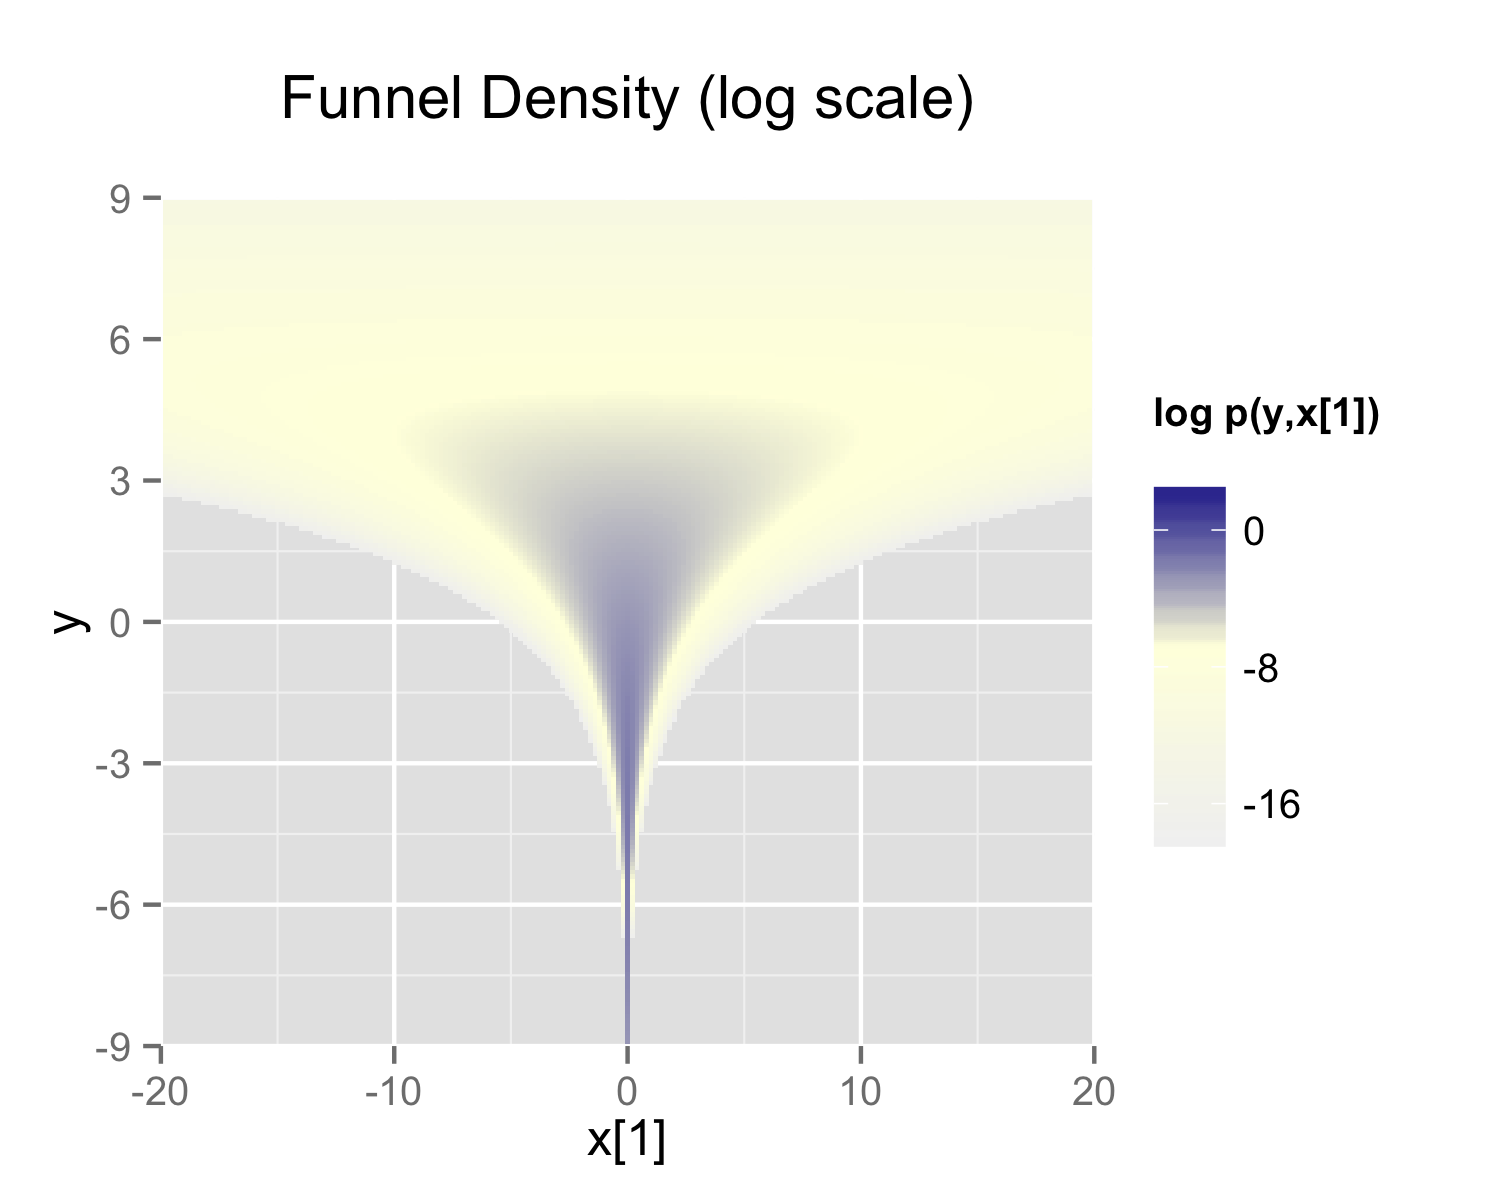
\includegraphics[height=2in]{R/funnel.png}
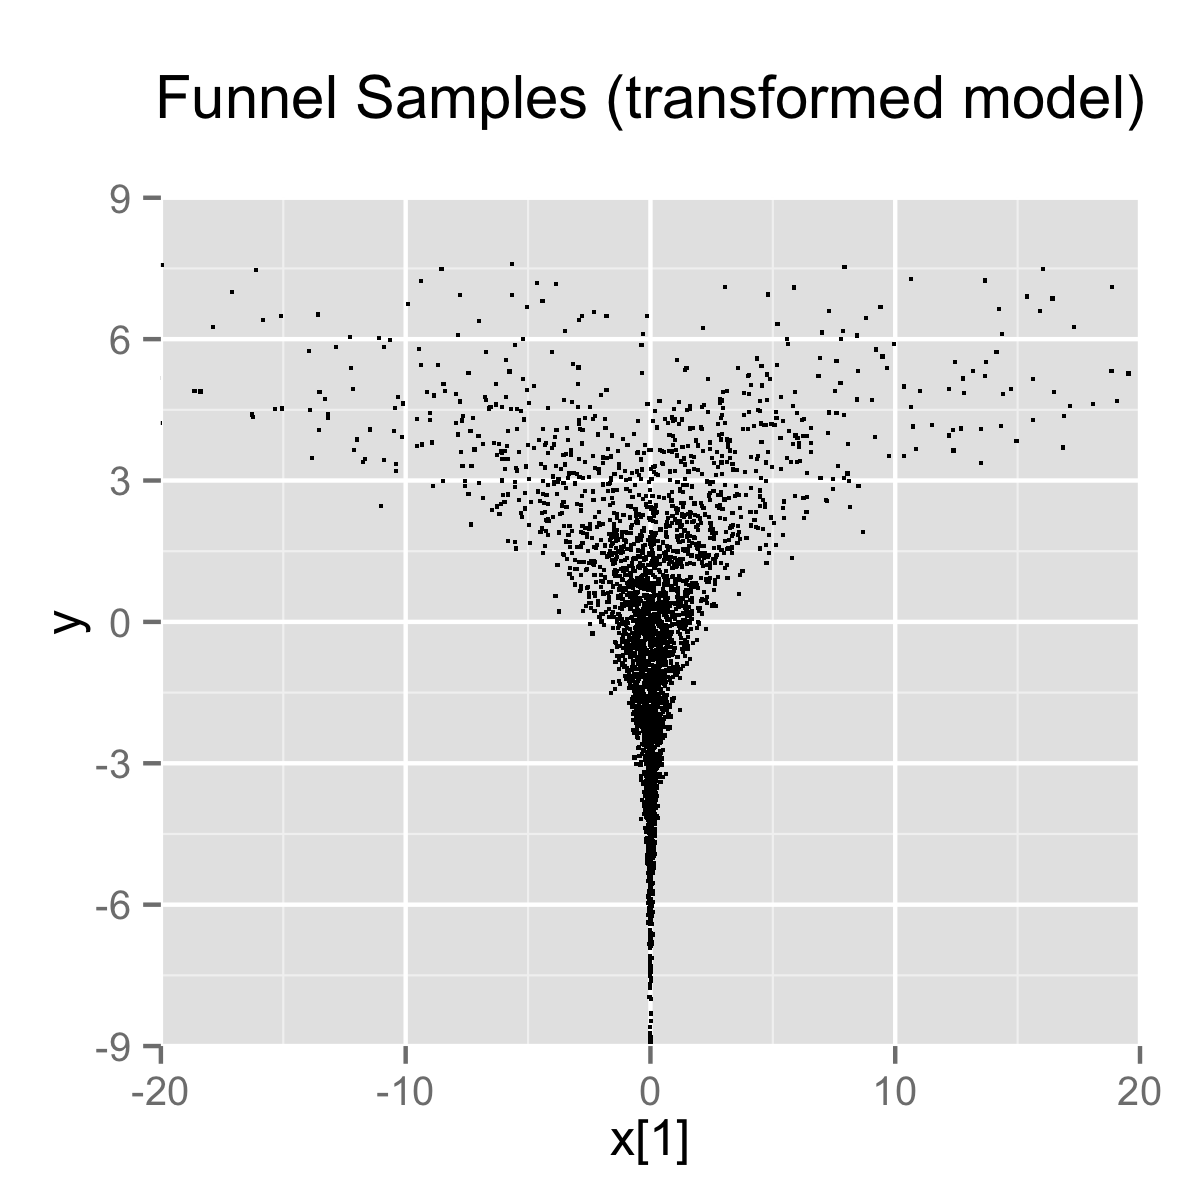
\includegraphics[height=2in]{R/funnel-fit.png}
\end{center}
\vspace*{-18pt}
\caption{\small \it Neal's Funnel.  (Left) The marginal density of
  Neal's funnel for the upper-level variable $y$ and one lower-level
  variable $x_1$ (see the text for the formula).  The blue region has
  log density greater than -8, the yellow region density greater than
  -16, and the gray background a density less than -16.  
  (Right) 4000 draws from a run of Stan's
  sampler with default settings.  Both plots are restricted to the
  shown window of $x_1$ and $y$ values; some draws fell outside of
  the displayed area as would be expected given the density.  The samples are
  consistent with the marginal density $p(y) =
  \distro{Normal}(y|0,3)$, which has mean 0 and standard deviation
  3.}\label{funnel.figure}
\end{figure}

\citep{Neal:2003} defines a distribution that exemplifies the
difficulties of sampling from some hierarchical models.  Neal's
example is fairly extreme, but can be trivially reparameterized in
such a way as to make sampling straightforward.

Neal's example has support for $y \in
\mathbb{R}$ and  $x \in \mathbb{R}^9$ with density
%
\[
p(y,x) = \distro{Normal}(y|0,3) \times \prod_{n=1}^9
\distro{Normal}(x_n|0,\exp(y/2)).
\]
%
The probability contours are shaped like ten-dimensional funnels.  The
funnel's neck is particularly sharp because of the exponential
function applied to $y$.  A plot of the log marginal density of $y$
and the first dimension $x_1$ is shown in \reffigure{funnel}.

The funnel can be implemented directly in Stan as follows.
%
\begin{quote}
\begin{Verbatim}
parameters {  
  real y;
  vector[9] x;
}
model {
  y ~ normal(0,3);
  x ~ normal(0,exp(y/2));
}
\end{Verbatim}
\end{quote}
%
When the model is expressed this way, Stan has trouble sampling from
the neck of the funnel, where $y$ is small and thus $x$ is constrained
to be near 0.  This is due to the fact that the density's scale
changes with $y$, so that a step size that works well in the body will
be too large for the neck and a step size that works in the neck will be
very inefficient in the body.

In this particular instance, because the analytic form of the density
from which samples are drawn is known, the model can be converted to
the following more efficient form.
%
\begin{quote}
\begin{Verbatim}
parameters {  
  real y_raw;
  vector[9] x_raw;
}
transformed parameters {
  real y;
  vector[9] x;

  y <- 3.0 * y_raw;  
  x <- exp(y/2) * x_raw;
}
model {
  y_raw ~ normal(0,1); // implies y ~ normal(0,3) 
  x_raw ~ normal(0,1); // implies x ~ normal(0,exp(y/2))  
}
\end{Verbatim}
\end{quote}
%
In this second model, the parameters \Verb|x_raw| and \Verb|y_raw| are
sampled as independent unit normals, which is easy for Stan.  These
are then transformed into samples from the funnel.  In this case, the
same transform may be used to define Monte Carlo samples directly
based on independent unit normal samples; Markov chain Monte Carlo
methods are not necessary. If such a reparameterization were used in
Stan code, it is useful to provide a comment indicating what the
distribution for the parameter implies for the distribution of the
transformed parameter.

\subsection{Reparameterizing the Cauchy}

Sampling from heavy tailed distributions such as the Cauchy is
difficult for Hamiltonian Monte Carlo, which operates within a
Euclidean geometry.%
\footnote{Riemann-manifold Hamiltonian Monte Carlo (RM-HMC) overcomes
  this difficulty by simulating the Hamiltonian dynamics in a a space
  with a position-dependent metric; see
  \citep{GirolamiCalderhead:2011} and \citep{Betancourt:2012}.}
%
The practical problem is that tail of the Cauchy
requires a relatively large step size compared to the trunk.  With a
small step size, the No-U-Turn sampler requires many steps when
starting in the tail of the distribution; with a large step size,
there will be too much rejection in the central portion of the
distribution.  This problem may be mitigated by defining the
Cauchy-distributed variable as the transform of a uniformly
distributed variable using the Cauchy inverse cumulative distribution
function.

Suppose a random variable of interest $X$ has a Cauchy distribution
with location $\mu$ and scale $\tau$, so that $X \sim
\distro{Cauchy}(\mu,\tau)$.  The variable $X$ has a cumulative
distribution function $F_X:\reals \rightarrow (0,1)$ defined by
\[
F_X(x) = \frac{1}{\pi} \arctan \left( \frac{x - \mu}{\tau} \right) +
\frac{1}{2}.
\]
The inverse of the cumulative distribution function,
$F_X^{-1}:(0,1) \rightarrow \reals$, is thus
%
\[
F^{-1}_X(y) = \mu + \tau \tan \left( \pi \left( x - \frac{1}{2} \right) \right).
\]
Thus if the random variable $Y$ has a unit uniform distribution, $Y
\sim \distro{Uniform}(0,1)$, then $F^{-1}_X(Y)$ has a Cauchy
distribution with location $\mu$ and scale $\tau$, i.e., $F^{-1}_X(Y) \sim
\distro{Cauchy}(\mu,\tau)$. 

Consider a Stan program involving a Cauchy-distributed parameter
\code{beta}.
%
\begin{quote}
\begin{Verbatim}
parameters {
  real beta;
  ...
}
model {
  beta ~ cauchy(mu,tau);
  ...
}
\end{Verbatim}
\end{quote}
%
This declaration of \code{beta} as a parameter may be replaced with a
transformed parameter \code{beta} defined in terms of a
uniform-distributed parameter \code{beta\_unif}.
%
\begin{quote}
\begin{Verbatim}
parameters {
  real<lower=-pi()/2, upper=pi()/2> beta_unif;
  ...
}
transformed parameters {
  real beta;
  beta <- mu + tau * tan(beta_unif);  // beta ~ cauchy(mu,tau)
}    
model {
  beta_unif ~ uniform(-pi()/2, pi()/2);  // not necessary
  ...
}
\end{Verbatim}
\end{quote}
%
It is more convenient in Stan to transform a uniform variable on
$(-\pi/2, \pi/2)$ than one on $(0,1)$.  The Cauchy location and scale
parameters, \code{mu} and \code{tau}, may be defined as data or may
themselves be parameters.  The variable \code{beta} could also be
defined as a local variable if it does not need to be included in the
sampler's output.

The uniform distribution on \code{beta\_unif} is defined explicitly in
the model block, but it could be safely removed from the program
without changing sampling behavior.  This is because $\log
\distro{Uniform}(\beta_{\mbox{\footnotesize unif}}|-\pi/2,\pi/2) =
-\log \pi$ is a constant and Stan only
needs the total log probability up to an additive constant.  Stan will spend
some time checking that that \code{beta\_unif} is between
\code{-pi()/2} and \code{pi()/2}, but this condition is guaranteed by
the constraints in the declaration of \code{beta\_unif}.  


\subsection{Hierarchical Models}

Unfortunately, the usual situation in applied Bayesian modeling
involves complex geometries and interactions that are not known
analytically.  Nevertheless, reparameterization can still be very
effective for separating parameters.  For example, a vectorized
hierarchical model might draw a vector of coefficients $\beta$ with
definitions as follows.
%
\begin{quote}
\begin{Verbatim}
parameters {
  real mu_beta;   
  real<lower=0> sigma_beta;
  vector[K] beta;
  ...
model {
  beta ~ normal(mu_beta,sigma_beta);
  ...
\end{Verbatim}
\end{quote}
%
Although not shown, a full model will have priors on both
\Verb|mu_beta| and \Verb|sigma_beta| along with data modeled based on
these coefficients.  For instance, a standard binary logistic
regression with data matrix \code{x} and binary outcome vector
\code{y} would include a likelihood statement such as form
\Verb|y ~ bernoulli_logit(x * beta)|, leading to an analytically
intractable posterior.

A hierarchical model such as the above will suffer from the same kind
of inefficiencies as Neal's funnel, though typically not so extreme,
because the values of \Verb|beta|, \Verb|mu_beta| and
\Verb|sigma_beta| are highly correlated in the posterior.  Such a
hierarchical model can be made much more efficient in terms of
effective sample size by reparameterizing in exactly the same way as
the funnel example.
%
\begin{quote}
\begin{Verbatim}
parameters {
  vector[K] beta_raw;
  ...
transformed parameters {
  vector[K] beta;
  // implies: beta ~ normal(mu_beta,sigma_beta)
  beta <- mu_beta + sigma_beta * beta_raw;
model {
  beta_raw ~ normal(0,1);  
  ...
\end{Verbatim}
\end{quote}
%
Any priors defined for \Verb|mu_beta| and \Verb|sigma_beta| remain as
defined in the original model.

Reparameterization of hierarchical models is not limited to the normal
distribution, although the normal distribution is the best candidate
for doing so. In general, any distribution of parameters in the 
location-scale family is a good candidate for reparameterization. Let
$\beta = l + s\alpha$ where $l$ is a location parameter and $s$ is a
scale parameter. Note that $l$ need not be the mean, $s$ need not
be the standard deviation, and neither the mean nor the standard
deviation need to exist. If $\alpha$ and $\beta$ are from the same
distributional family but $\alpha$ has location zero and unit scale, 
while $\beta$ has location $l$ and scale $s$, then that distribution
is a location-scale distribution. Thus, if $\alpha$ were a parameter
and $\beta$ were a transformed parameter, then a prior distribution
from the location-scale family on $\alpha$ with location zero and unit 
scale implies a prior distribution on $\beta$ with location $l$ and
scale $s$. Doing so would reduce the dependence between $\alpha$, 
$l$, and $s$.

There are several univariate distributions in the location-scale
family, such as the Student t distribution, including its special
cases of the Cauchy distribution (with one degree of freedom) and the
normal distribution (with infinite degrees of freedom). As shown above,
if $\alpha$ is distributed standard normal, then $\beta$ is distributed
normal with mean $\mu = l$ and standard deviation $\sigma = s$. The 
logistic, the double exponential, the generalized extreme value 
distributions, and the stable distribution are also in the 
location-scale family.

Also, if $z$ is distributed standard normal, then $z^2$ is distributed
chi-squared with one degree of freedom. By summing the squares of $K$
independent standard normal variates, one can obtain a single variate
that is distributed chi-squared with $K$ degrees of freedom. However,
for large $K$, the computational gains of this reparameterization may
be overwhelmed by the computational cost of specifying $K$ primitive
parameters just to obtain one transformed parameter to use in a model.

\subsection{Multivariate Reparameterizations}

The benefits of reparameterization are not limited to univariate 
distributions. A parameter with a multivariate normal prior distribution
is also an excellent candidate for reparameterization. Suppose you intend
the prior for $\beta$ to be multivariate normal with mean vector $\mu$
and covariance matrix $\Sigma$. Such a belief is reflected by the
following code.
%
\begin{quote}
\begin{Verbatim}
data {
  int<lower=2> K;
  vector[K] mu;
  cov_matrix[K] Sigma;
  ...
parameters {
  vector[K] beta;
  ...
model {
  beta ~ multi_normal(mu,Sigma);
  ...
\end{Verbatim}
\end{quote}
%
In this case \Verb|mu| and \Verb|Sigma| are fixed data, but they could
be unknown parameters, in which case their priors would be unaffected
by a reparameterization of \Verb|beta|.

If $\alpha$ has the same dimensions as $\beta$ but the elements of 
$\alpha$ are independently and identically distributed standard normal 
such that $\beta = \mu + L\alpha$, where $LL^\top = \Sigma$, then 
$\beta$ is distributed multivariate normal with mean vector $\mu$ and 
covariance matrix $\Sigma$. One choice for $L$ is the Cholesky factor
of $\Sigma$. Thus, the model above could be reparameterized as follows.
%
\begin{quote}
\begin{Verbatim}
data {
  int<lower=2> K;
  vector[K] mu;
  cov_matrix[K] Sigma;
  ...
transformed data {
  matrix[K,K] L;
  L <- cholesky_decompose(Sigma);
}
parameters {
  vector[K] alpha;
  ...
transformed parameters {
  vector[K] beta;
  beta <- mu + L * alpha; 
}
model {
  alpha ~ normal(0,1); 
  // implies: beta ~ multi_normal(mu, Sigma)
  ...
\end{Verbatim}
\end{quote}
%
This reparameterization is more efficient for two reasons. First, it
reduces dependence among the elements of \Verb|alpha| and second, it
avoids the need to invert \Verb|Sigma| every time \Verb|multi_normal|
is evaluated.

The Cholesky factor is also useful when a covariance matrix is 
decomposed into a correlation matrix that is multiplied from both
sides by a diagonal matrix of standard deviations, where either the
standard deviations or the correlations are unknown parameters. The
Cholesky factor of the covariance matrix is equal to the product of
a diagonal matrix of standard deviations and the Cholesky factor of
the correlation matrix. Furthermore, the product of a diagonal matrix
of standard deviations and a vector is equal to the elementwise
product between the standard deviations and that vector. Thus, if for
example the correlation matrix \Verb|Tau| were fixed data but the
vector of standard deviations \Verb|sigma| were unknown parameters,
then a reparameterization of \Verb|beta| in terms of \Verb|alpha|
could be implemented as follows.
%
\begin{quote}
\begin{Verbatim}
data {
  int<lower=2> K;
  vector[K] mu;
  corr_matrix[K] Tau;
  ...
transformed data {
  matrix[K,K] L;
  L <- cholesky_decompose(Tau);
}
parameters {
  vector[K] alpha;
  vector<lower=0>[K] sigma;
  ...
transformed parameters {
  vector[K] beta;
  // This equals mu + diag_matrix(sigma) * L * alpha;
  beta <- mu + sigma .* (L * alpha);
}
model {
  sigma ~ cauchy(0,5);
  alpha ~ normal(0,1);
  // implies: beta ~ multi_normal(mu,
  //  diag_matrix(sigma) * L * L' * diag_matrix(sigma)))
  ...
\end{Verbatim}
\end{quote}
%
This reparameterization of a multivariate normal distribution in
terms of standard normal variates can be extended to other multivariate
distributions that can be conceptualized as contaminations of the 
multivariate normal, such as the multivariate Student t and the skew
multivariate normal distribution.

A Wishart distribution can also be reparameterized in terms of standard
normal variates and chi-squared variates. Let $L$ be the Cholesky factor
of a $K \times K$ positive definite scale matrix $S$ and let $\nu$ be
the degrees of freedom. If
\begin{equation*}
A = \left( \begin{array}{cccc}
\sqrt{c_{1}} & 0 & \cdots & 0\\
z_{21} & \sqrt{c_{2}} & \ddots & \vdots\\
\vdots & \ddots & \ddots & 0\\
z_{K1} & \cdots & z_{K\left(K-1\right)} & \sqrt{c_{K}}
 \end{array} \right),
\end{equation*}
where each $c_i$ is distributed chi-squared with $\nu - i + 1$ degrees
of freedom and each $z_{ij}$ is distributed standard normal, then
$W = LAA^{\top}L^{\top}$ is distributed Wishart with scale matrix
$S = LL^{\top}$ and degrees of freedom $\nu$. Such a reparameterization
can be implemented by the following Stan code:
%
\begin{quote}
\begin{Verbatim}
data {
  int<lower=1> N;
  int<lower=1> K;
  int<lower=K+2> nu
  matrix[K,K] L; // Cholesky factor of scale matrix
  vector[K] mu;
  matrix[N,K] y;
  ...
parameters {
  vector<lower=0>[K] c;
  vector[0.5 * K * (K - 1)] z;
  ...
model {
  matrix[K,K] A;
  int count;
  count <- 1;
  for (j in 1:K) {
    for (i in (j+1):K) {
      A[i,j] <- z[count];
      count <- count + 1;
    }
    for (i in 1:(j - 1)) {
      A[i,j] <- 0.0;
    }
    A[j,j] <- sqrt(c[j]);
  }
  
  for (i in 1:K) {
    c[i] ~ chi_square(nu - i + 1);
  }
  z ~ normal(0,1);
  // implies: L * A * A' * L' ~ wishart(nu, L * L')
  y ~ multi_normal_cholesky(mu, L * A);
  ...
\end{Verbatim}
\end{quote}
%
This reparameterization is more efficient for three reasons. First, it
reduces dependence among the elements of \Verb|z| and second, it
avoids the need to invert the covariance matrix, $W$ every time 
\Verb|wishart| is evaluated. Third, if $W$ is to be used with a
multivariate normal distribution, you can pass $L A$ to the more
efficient \Verb|multi_normal_cholesky| function, rather than passing
$W$ to \Verb|multi_normal|.

If $W$ is distributed Wishart with scale matrix $S$ and degrees of
freedom $\nu$, then $W^{-1}$ is distributed inverse Wishart with inverse
scale matrix $S^{-1}$ and degrees of freedom $\nu$. Thus, the previous
result can be used to reparameterize the inverse Wishart distribution.
Since $W = L * A * A^{\top} * L^{\top}$, 
$W^{-1} = L^{{\top}^{-1}} A^{{\top}^{-1}} A^{-1} L^{-1}$, where all four
inverses exist, but 
$L^{{-1}^{\top}} = L^{{\top}^{-1}}$ and $A^{{-1}^{\top}} = A^{{\top}^{-1}}$.
We can slightly modify the above Stan code for this case:
%
\begin{quote}
\begin{Verbatim}
data {
  int<lower=1> K;
  int<lower=K+2> nu
  matrix[K,K] L; // Cholesky factor of scale matrix
  ...
transformed data {
  matrix[K,K] eye;
  matrix[K,K] L_inv;
  for (j in 1:K) {
    for (i in 1:K) {
      eye[i,j] <- 0.0;
    }
    eye[j,j] <- 1.0;
  }
  L_inv <- mdivide_left_tri_low(L, eye);
}
parameters {
  vector<lower=0>[K] c;
  vector[0.5 * K * (K - 1)] z;
  ...
model {
  matrix[K,K] A;
  matrix[K,K] A_inv_L_inv;  
  int count;
  count <- 1;
  for (j in 1:K) {
    for (i in (j+1):K) {
      A[i,j] <- z[count];
      count <- count + 1;
    }
    for (i in 1:(j - 1)) {
      A[i,j] <- 0.0;
    }
    A[j,j] <- sqrt(c[j]);
  }
  A_inv_L_inv <- mdivide_left_tri_low(A, L_inv);
  for (i in 1:K) {
    c[i] ~ chi_square(nu - i + 1);
  }
  z ~ normal(0,1); // implies: crossprod(A_inv_L_inv) ~ 
  // inv_wishart(nu, L_inv' * L_inv)
  ...
\end{Verbatim}
\end{quote}
%
Another candidate for reparameterization is the Dirichlet distribution
with all $K$ shape parameters equal. \cite{ZyczkowskiSommers:2001} shows 
that if $\theta_i$ is equal to the sum of $\beta$ independent squared 
standard normal variates and $\rho_i = \frac{\theta_i}{\sum \theta_i}$, 
then the $K$-vector $\rho$ is distributed Dirichlet with all shape 
parameters equal to $\frac{\beta}{2}$. In particular, if $\beta = 2$, 
then $\rho$ is distributed uniformally on the unit simplex. Thus, we can 
make $\rho$ be a transformed parameter to reduce dependence, as in:
%
\begin{quote}
\begin{Verbatim}
data {
  int<lower=1> beta;
  ...
parameters {
  vector[beta] z[K];
  ...
transformed parameters {
  simplex[K] rho;
  for (k in 1:K)
    rho[k] <- dot_self(z[k]); // sum-of-squares
  rho <- rho / sum(rho);
}
model {
  for (k in 1:K)
    z[k] ~ normal(0,1); 
  // implies: rho ~ dirichlet(0.5 * beta * ones)
  ...
\end{Verbatim}
\end{quote}
%

\section{Vectorization}

\subsection{Gradient Bottleneck}

\Stan spends the vast majority of its time computing the gradient of
the log probability function, making gradients the obvious target for
optimization.  \Stan's gradient calculations with algorithmic
differentiation require a template expression to be allocated%
%
\footnote{\Stan uses its own arena-based allocation, so allocation and
  deallocation are faster than with a raw call to \code{new}.}
%
and constructed for each subexpression of a \Stan program involving
parameters or transformed parameters.  This section defines
optimization strategies based on vectorizing these subexpressions to
reduce the work done during algorithmic differentiation.

\subsection{Vectorizing Summations}

Because of the gradient bottleneck described in the previous section,
it is more efficient to collect a sequence of summands into a vector
or array and then apply the \code{sum()} operation than it is to
continually increment a variable by assignment and addition.  For
example, consider the following code snippet, where \code{foo()} is
some operation that depends on \code{n}.
%
\begin{quote}
\begin{Verbatim}
for (n in 1:N) 
   total <- total + foo(n,...);
\end{Verbatim}
\end{quote}
%
This code has to create intermediate representations for each
of the \code{N} summands.  

A faster alternative is to copy the values into a vector, then
apply the \code{sum()} operator, as in the following refactoring.
%
\begin{quote}
\begin{Verbatim}
{  
  vector[N] summands;
  for (n in 1:N) 
    summands[n] <- foo(n,...);
  total <- sum(summands);
}
\end{Verbatim}
\end{quote}
%
Syntactically, the replacement is a statement block delineated
by curly brackets (\Verb|{|, \Verb|}|), starting with the definition
of the local variable \code{summands}.

Even though it involves extra work to allocate the \code{summands}
vector and copy \code{N} values into it, the savings in
differentiation more than make up for it.  Perhaps surprisingly,
it will also use substantially less memory overall than incrementing
\code{total} within the loop.


\subsection{Vectorization through Matrix Operations}

The following program directly encodes a linear regression with fixed
unit noise using a two-dimensional array \code{x} of predictors, an
array \code{y} of outcomes, and an array \code{beta} of regression
coefficients.
%
\begin{quote}
\begin{Verbatim}
data {
    int<lower=1> K;
    int<lower=1> N;
    real x[K,N];
    real y[N];
}
parameters {
    real beta[K];
}
model {
    for (n in 1:N) {
        real gamma;  gamma <- 0.0;
        for (k in 1:K)
            gamma <- gamma + x[n,k] * beta[k];
        y[n] ~ normal(gamma,1);
    }
}
\end{Verbatim}
\end{quote}
%
The following model computes the same log probability function as the
previous model, even supporting the same input files for data and
initialization.
%
\begin{quote}
\begin{Verbatim} 
data {
    int<lower=1> K;
    int<lower=1> N;
    vector[K] x[N];
    real y[N];
}
parameters {
    vector[K] beta;
}
model {
    for (n in 1:N)
        y[n] ~ normal(dot_product(x[n],beta), 1);
}
\end{Verbatim}
\end{quote}
%
Although it produces equivalent results, the dot product should not be
replaced with a transpose and multiply, as in
%
\begin{quote}
\begin{Verbatim} 
        y[n] ~ normal(x[n]' * beta, 1);
\end{Verbatim}
\end{quote}
%
The relative inefficiency of the transpose and multiply approach is
that the transposition operator allocates a new vector into which the
result of the transposition is copied.  This consumes both time
and memory\footnote{Future versions of \Stan may remove this inefficiency
by more fully exploiting expression templates inside the Eigen
\Cpp matrix library.  This will require enhancing Eigen to deal
with mixed-type arguments, such as the type \code{double} used
for constants and the algorithmic differentiation type
\code{stan::agrad::var} 
used for variables.}.
%
The inefficiency of transposition could itself be mitigated somewhat by
reordering the product and pulling the transposition out of the loop,
as follows.
%
\begin{quote}
\begin{Verbatim} 
...
transformed parameters {
    row_vector[K] beta_t;
    beta_t <- beta';
}
model {
    for (n in 1:N)
        y[n] ~ normal(beta_t * x[n], 1);
}
\end{Verbatim}
\end{quote}
%
The problem with transposition could be completely solved by directly
encoding the \code{x} as a row vector, as in the
following example.
%
\begin{quote}
\begin{Verbatim} 
data {
    ...
    row_vector[K] x[N];
    ...
}
parameters {
    vector[K] beta;
}
model {
    for (n in 1:N)
        y[n] ~ normal(x[n] * beta, 1);
}
\end{Verbatim}
\end{quote}
%
Declaring the data as a matrix and then computing all the predictors
at once using matrix multiplication is more efficient still, as in the
example discussed in the next section.

\subsection{Vectorized Probability Functions}

The final and most efficient version replaces the loops and
transformed parameters by using the vectorized form of the normal
probability function, as in the following example.
%
\begin{quote}
\begin{Verbatim} 
data {
    int<lower=1> K;
    int<lower=1> N;
    matrix[N,K] x;
    vector[N] y;
}
parameters {
    vector[K] beta;
} 
model {
    y ~ normal(x * beta, 1);
}
\end{Verbatim}
\end{quote}
%
The variables are all declared as either matrix or vector types.
The result of the matrix-vector multiplication \code{x * beta} in the
model block is a vector of the same length as \code{y}.  

The probability function documentation in \refpart{built-in-functions}
indicates which of \Stan's probability functions support
vectorization; see \refsection{prob-vectorization} for more
information.  Vectorized probability functions accept either vector or
scalar inputs for all arguments, with the only restriction being that
all vector arguments are the same dimensionality.  In the example
above, \code{y} is a vector of size \code{N}, \code{x * beta} is a
vector of size \code{N}, and \code{1} is a scalar.

\section{Exploiting Sufficient Statistics}

In some cases, models can be recoded to exploit sufficient statistics
in estimation.  This can lead to large efficiency gains compared to an
expanded model.  For example, consider the following Bernoulli
sampling model.
%
\begin{quote}
\begin{Verbatim}
data {
    int<lower=0> N;
    int<lower=0,upper=1> y[N];
    real<lower=0> alpha;
    real<lower=0> beta;
}
parameters {
    real<lower=0,upper=1> theta;
}
model {
    theta ~ beta(alpha,beta);
    for (n in 1:N) 
        y[n] ~ bernoulli(theta);
}
\end{Verbatim}
\end{quote}
%
In this model, the sum of positive outcomes in \code{y} is a
sufficient statistic for the chance of success \code{theta}.  The
model may be recoded using the binomial distribution as follows.
%
\begin{quote}
\begin{Verbatim}
    theta ~ beta(alpha,beta);
    sum(y) ~ binomial(N,theta);
\end{Verbatim}
\end{quote}
%
Because truth is represented as one and falsehood as zero, the sum
\code{sum(y)} of a binary vector \code{y} is equal to the number of
positive outcomes out of a total of \code{N} trials.  



\section{Exploiting Conjugacy}


Continuing the model from the previous section, the conjugacy of the
beta prior and binomial sampling distribution allow the model to be
further optimized to the following equivalent form.
%
\begin{quote}
\begin{Verbatim}
    theta ~ beta(alpha + sum(y), beta + N - sum(y));
\end{Verbatim}
\end{quote}
%
To make the model even more efficient, a transformed data variable
defined to be \code{sum(y)} could be used in the place of \code{sum(y)}.


% \section{Using Forward Sampling}

% In fact, at this point, simple (non Markov chain) Monte Carlo may be
% used because the parameters to the beta distribution are specified and
% there are no variables that depend on \code{theta}.  Thus this model
% could be even further optimized by replacing the declaration of
% \code{theta} as a parameter with a declaration as a generated quantity
% and then generating the quantity directly.
% %
% \begin{quote}
% \begin{Verbatim}
% generated quantities {
%     real<lower=0,upper=1> theta;
%     theta ~ random_beta(alpha + sum(y), beta + N - sum(y));
% }
% \end{Verbatim}
% \end{quote}
% %
% When used in the generated quantities block, sampling statements such
% as that for \code{theta} are executed by taking a sample from the
% specified distribution directly. The result is a Monte Carlo estimate
% of \code{theta} in which every sample is independent (up to the limits
% of the pseudorandom number generator, of course).  Thus the effective
% sample size should be estimated as being roughly equal to the sample
% size.
